\bigskip
\section{Simulations}

\subsection{Chosen parameters}

In regards of the simulation scenarios we are deliberately neglecting the
critical aspects of the communication between master and slave.

Therefore all the following simulations has been run assuming ideal conditions as an
instantaneous and loss-less signal transfer between master and slave subsystems.

\bigskip

\begin{table}[H]
\centering
	\begin{tabular}{c c c c}
		\toprule
		Symbol & Parameter & Value & Unit\\
		\midrule 
		\midrule 
    & \textsl{Master-Slave system}\\
		\midrule 
		$J_{m}$  & Master Inertia & $5\cdot 10^{-4}$ & $\text{kg}\cdot \text{m\textsuperscript{2}}$ \\
		$J_{s}$  & Slave Inertia & $5\cdot 10^{-4}$ & $\text{kg}\cdot \text{m\textsuperscript{2}}$ \\
    \midrule 
    & \textsl{Desired cut-off frequencies}\\
		\midrule 
		$g_{1}$  & 1\textsuperscript{st} cut-off frequency & $5\cdot 10^{1}$ & rad/s \\
		$g_{2}$  & 2\textsuperscript{nd} cut-off frequency & $5\cdot 10^{2}$ & rad/s \\
		\bottomrule
	\end{tabular}
	\caption{Parameters adopted in simulations.}
	\label{simParams}
\end{table}

\bigskip

The table n.\ref{simParams} describes the parameters chosen such as inertiae and
cut-off frequencies, consequently the table n.\ref{virtParams} describes
the virtual coefficients computed as explained in section \ref{ParamSelect}.

\bigskip

\begin{table}[H]
\centering
	\begin{tabular}{c c c c}
		\toprule
		Behaviour & $K_{v}$ & $B_{v}$ &  $J_{v}$\\
		\midrule 
		\midrule 
	    Virtual compliance& $20.0 \ \frac{\text{N m}}{\text{rad}} $ & $4.4\cdot 10^{-1} \ \frac{\text{N m}}{\text{rad/s}}$ & $3\cdot 10^{-4} \ \text{kg m\textsuperscript{2}}$\\
    	Rigid coupling & $10^{2} \ \frac{\text{N m}}{\text{rad}} $ & $1.5\cdot 10^{-1} \ \frac{\text{N m}}{\text{rad/s}}$ & $ 0 \ \text{kg m\textsuperscript{2}} $\\
		\bottomrule
	\end{tabular}
	\caption{Sets of chosen virtual parameters.}
	\label{virtParams}
\end{table}
\newpage

\subsection{Disturbance rejection performances}

We consider at first the rigid coupling case, in which, as being said, almost
full transparency is achieved between master and slave. The vibrations
transmitted by the environment on the slave-side will be felt almost with the same intensity on the master-side whatever would be the vibration frequency.

\begin{figure}[h]
	\centering
	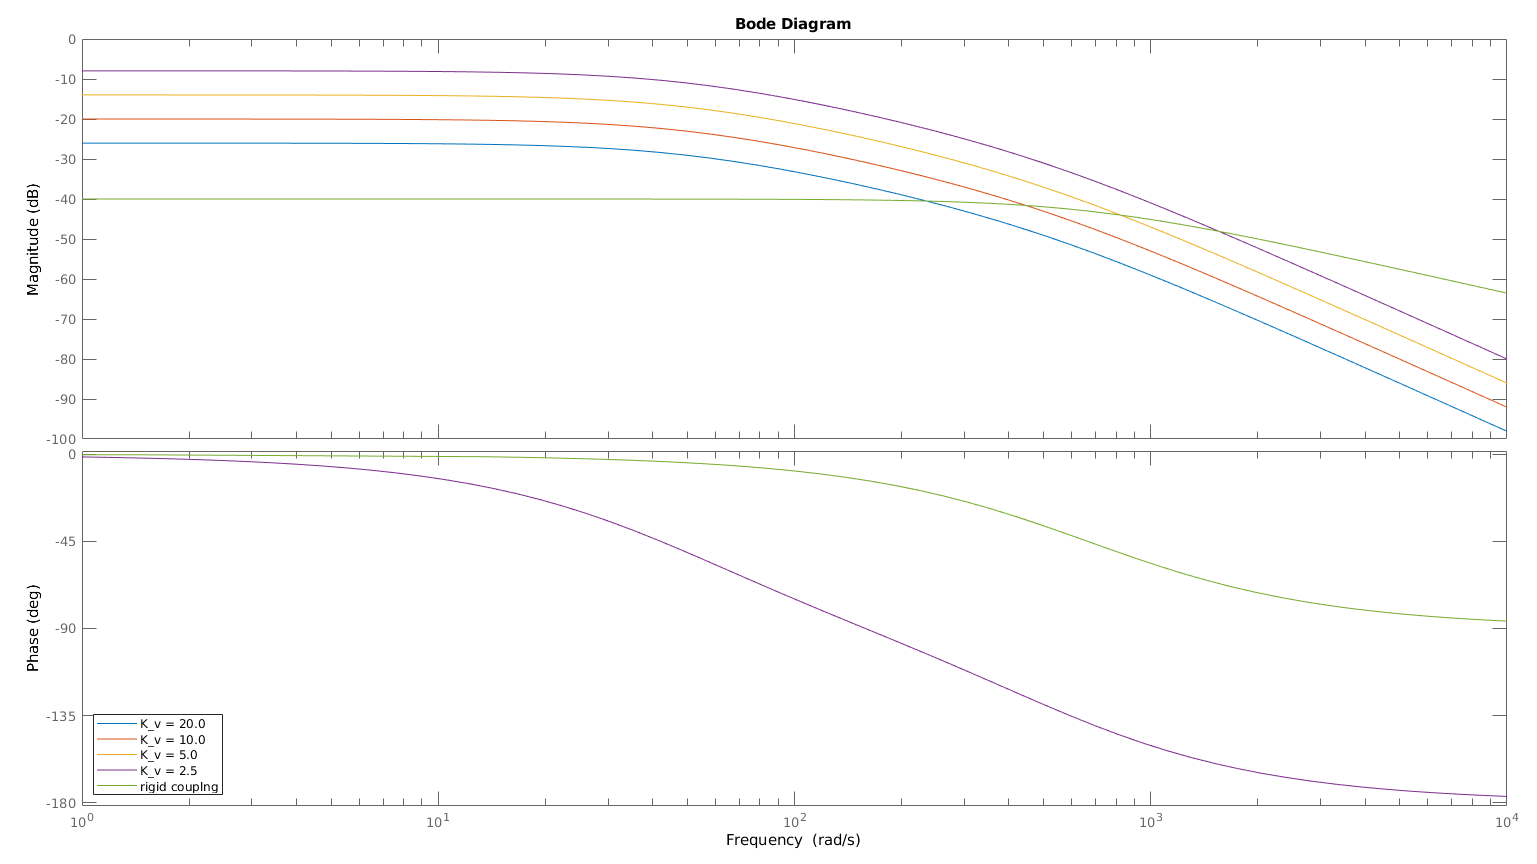
\includegraphics[width=1\linewidth]{Images/bodo}
	\caption{Frequency response relative to $ H_{22} $ hybrid parameter.}
	\label{fig:bodo}
\end{figure}

For this reason, in order to reach better task execution performances we want to
reduce the impact of environment vibrations at minimum.

The simulations aims to compare two opposite behaviours: \textbf{rigid coupling}
and \textbf{induced virtual compliance}, achieved through the choice of
the desired cut-off frequencies.

Fig.\ref{fig:bodo} describes the frequency response of the function \eqref{H_22} with several virtual parameters sets, defined starting from different spring stiffness values $ K_v $ varying from $ 2.5 \ \text{N}\cdot\text{m}/\text{rad} $ to $ 20 \ \text{N}\cdot\text{m}/\text{rad} $, and the rigid coupling control set.

At low frequencies the signals are preserved in both the rigid coupling and the virtual compliance controls. In particular, the magnitude of the response increases with inverse of the virtual spring stiffness, describing the \textbf{compliance} of the system. At high frequencies the disturbance rejection is exerted more effectively by the virtual compliance control: the position response to high frequency external torque is reduced due to the low compliance.

%This could be accomplished, as shown before, by building an ad-hoc filter, such
%as fig.\ref{fig:bodo} depicits, in which there are different slope profiles that
%will end up rejecting the disturbances at higher frequencies than the
%\textsl{cut-off} ones and preserving the signal at lower ones.

%The simulations aims to compare two opposite behaviours: \textbf{rigid coupling}
%and \textbf{induced virtual compliance} which is achieved through the choice of
%the desired cut-off frequencies.
%\newline

%Another description of the frequency response of the system is provided by the figs.\ref{positionResponceFrequencies}

%In particular these frequencies correspond respectively to 8 and 80 Hz.
It is interesting the comparison of the vibration suppression applied on three
different input frequencies, as shown in figs.\ref{positionResponceFrequencies}
\footnote{For the sake of simplicity the different control set are called:
	\begin{itemize}
		\item Control set 1 : defined by $ K_v = 2.5 \frac{\text{N} \cdot \text{m}}{\text{rad}}$;
		\item Control set 2 : defined by $ K_v = 5.0 \frac{\text{N} \cdot \text{m}}{\text{rad}}$;
		\item Control set 3 : defined by $ K_v = 10.0 \frac{\text{N} \cdot \text{m}}{\text{rad}}$;
		\item Control set 4 : defined by $ K_v = 20.0 \frac{\text{N} \cdot \text{m}}{\text{rad}}$.	
\end{itemize}
}:

\begin{itemize}
%\item $10^{1} Hz$ : In fig.\ref{fig:10Htz} is shown how the vibrations at lower frequencies are preserved by the\textsl{virtual compliance}, this is a rather enticing aspect of a teleoperation interaction since the input commands generated by the controller will have kind of low frequencies.
\item $ 10 \ \text{Hz} $ input : in fig.\ref{fig:10Htz} is shown how the inputs at lower frequencies are preserved by the \textbf{control set 4} (defined by $ K_v = 2.5 \ \text{N}\cdot\text{m/s} $). The response is less large as stiffness increases. The phase is almost the same for virtual compliance and rigid coupling controls;
%\item $10^{2} \text{Hz}$ : The fig.\ref{fig:100Htz} demonstrates a turning point in which the disturbance rejection achieved by the \textsl{rigid coupling} is comparable to the performance of \textsl{virtual compliance}.
\item $10^{2} \ \text{Hz}$ input : as before the response decreases as the virtual spring stiffness increase. The difference here is the almost the same response of the \textbf{control set 1} ($ K_v = 20 \ \text{N}\cdot\text{m/s} $) and the rigid coupling ($ K_v = 10^2 \ \text{N}\cdot\text{m/s} $), despite the second one is defined by a larger value of stiffness. The phase relative to the \textbf{control sets} is delayed respect to the rigid coupling control (fig.\ref{fig:100Htz});
\item $10^{3} \ \text{Hz}$ input : at frequencies higher than the cut-off ones, the
inputs are dumped more effectively by the \textbf{control sets} than the \textbf{rigid coupling control}, for which we have larger response (fig.\ref{fig:1000Htz}).
\end{itemize}

\begin{figure}[H]
	\begin{subfigure}[h!]{1\linewidth}
		\centering
		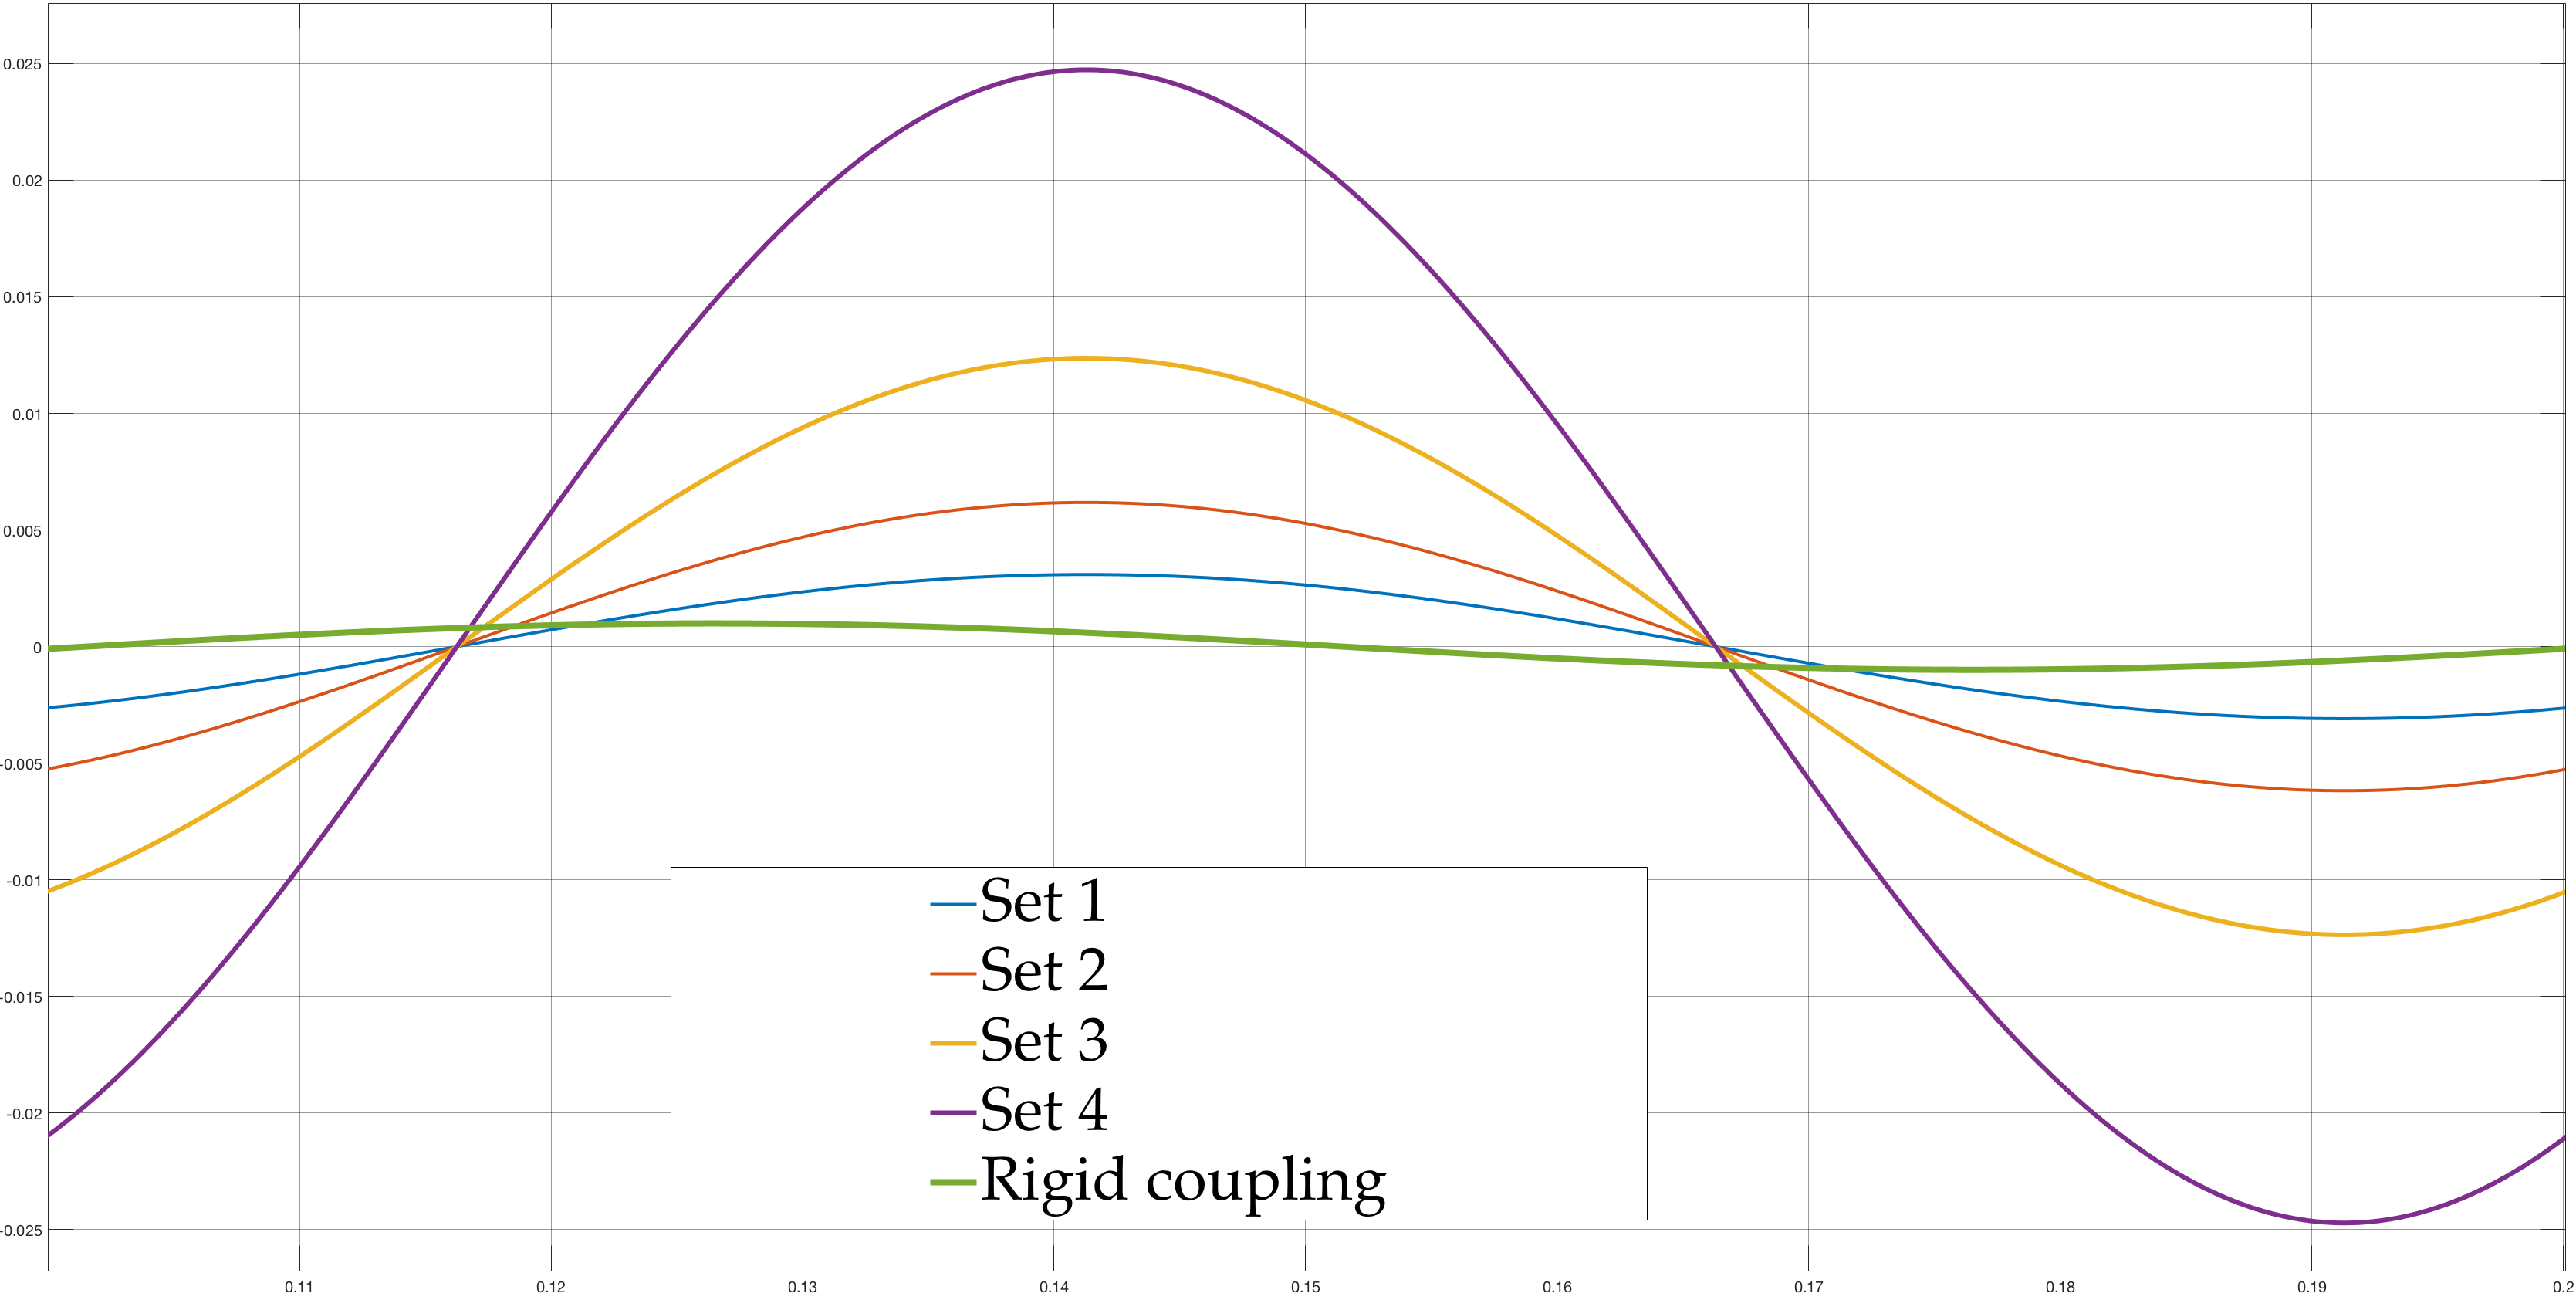
\includegraphics[width=\textwidth, height=0.29\textwidth]{Images/vibr10Htz}
		\caption{10 Hz}
		\label{fig:10Htz}
	\end{subfigure}
\end{figure}
\begin{figure}\ContinuedFloat
	\begin{subfigure}[h!]{1\linewidth}
		\centering
		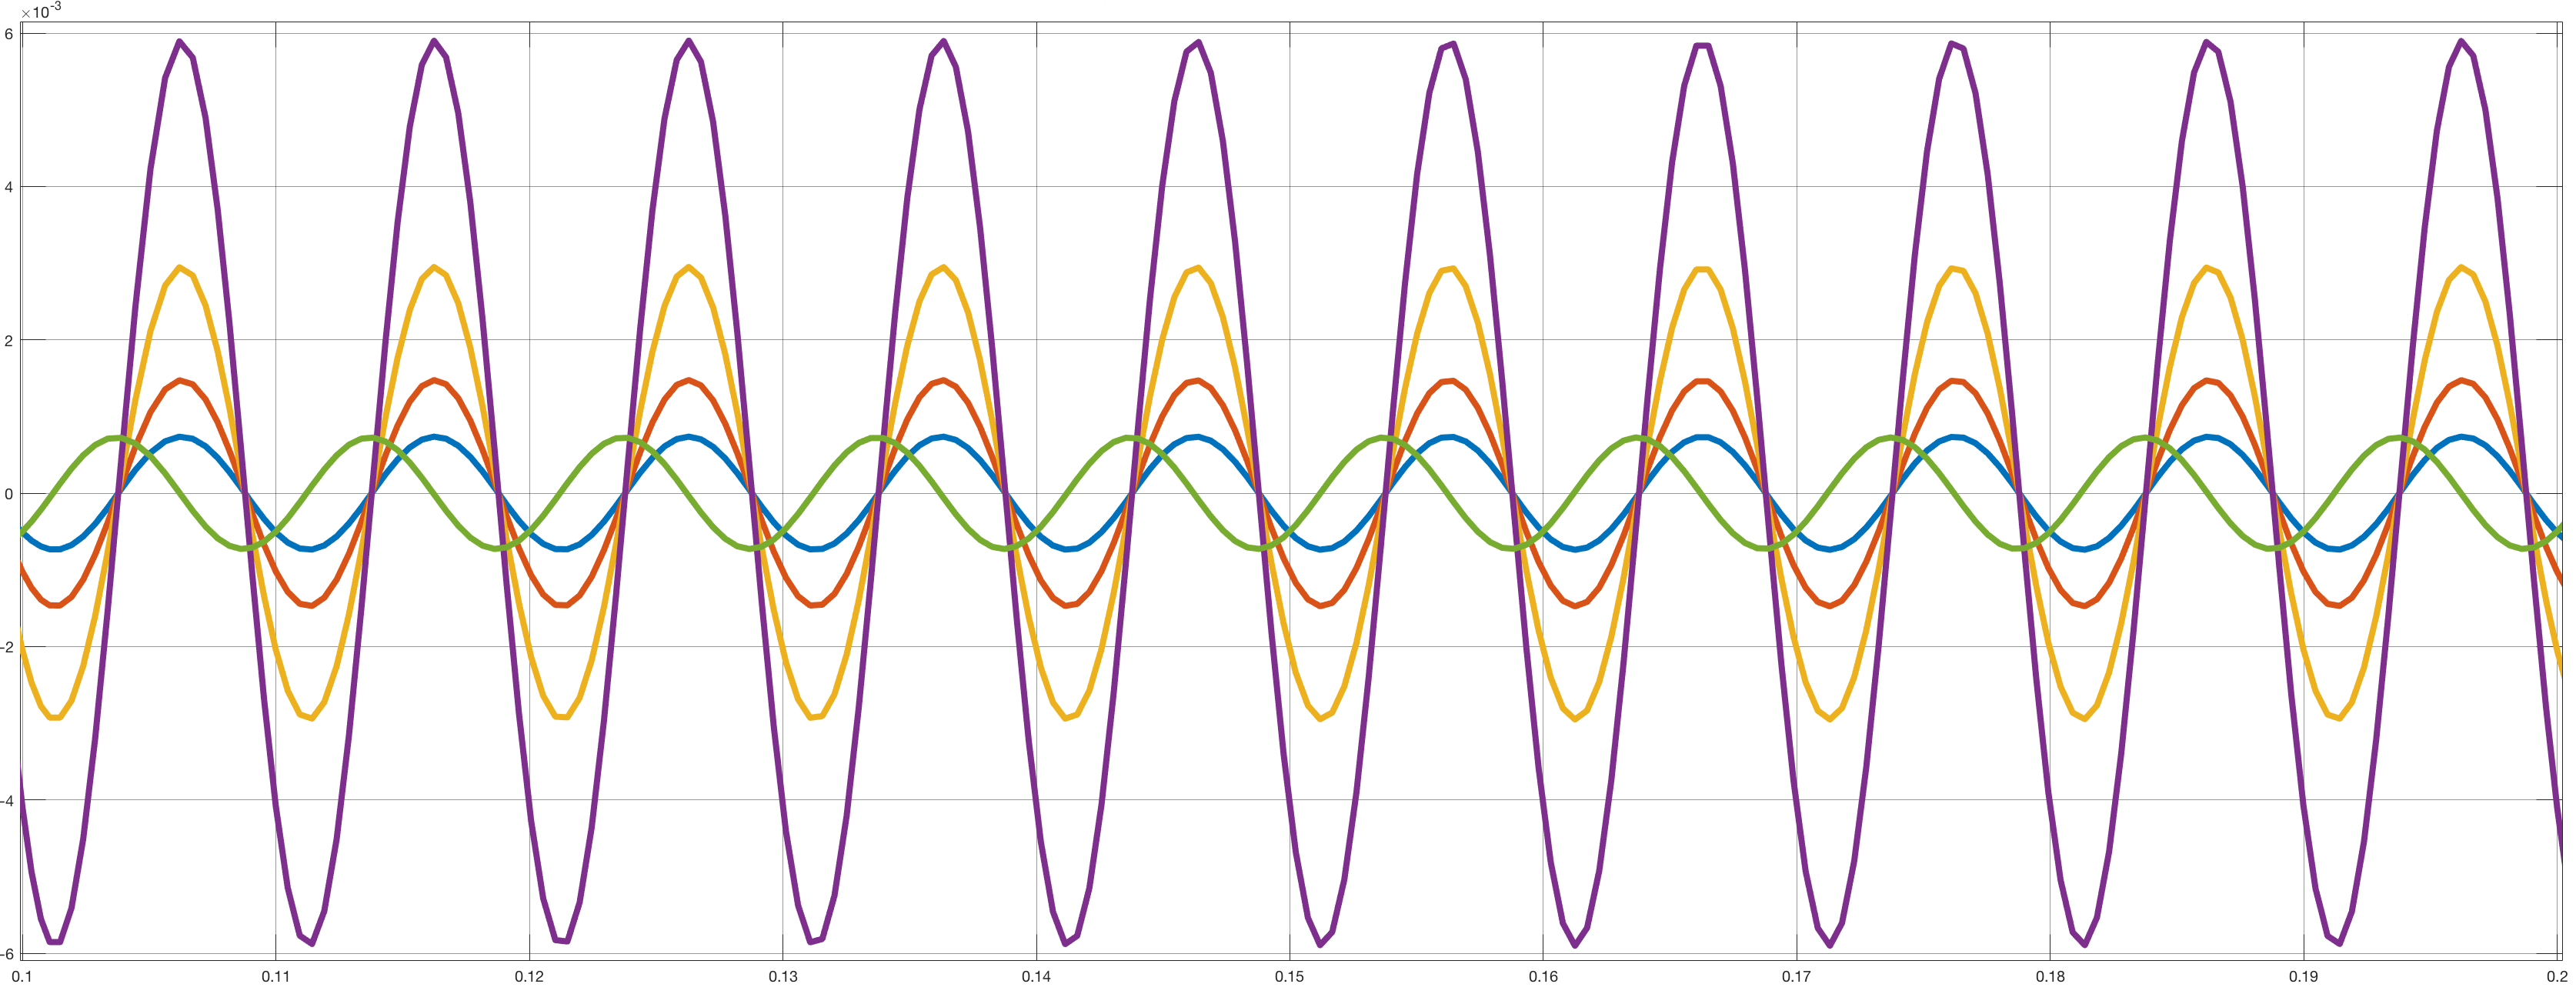
\includegraphics[width=\textwidth, height=0.29\textwidth]{Images/vibr100Htz}
		\caption{100 Hz}
		\label{fig:100Htz}
	\end{subfigure}
\end{figure}
\begin{figure}\ContinuedFloat
	\begin{subfigure}[h!]{1\linewidth}
		\centering.
		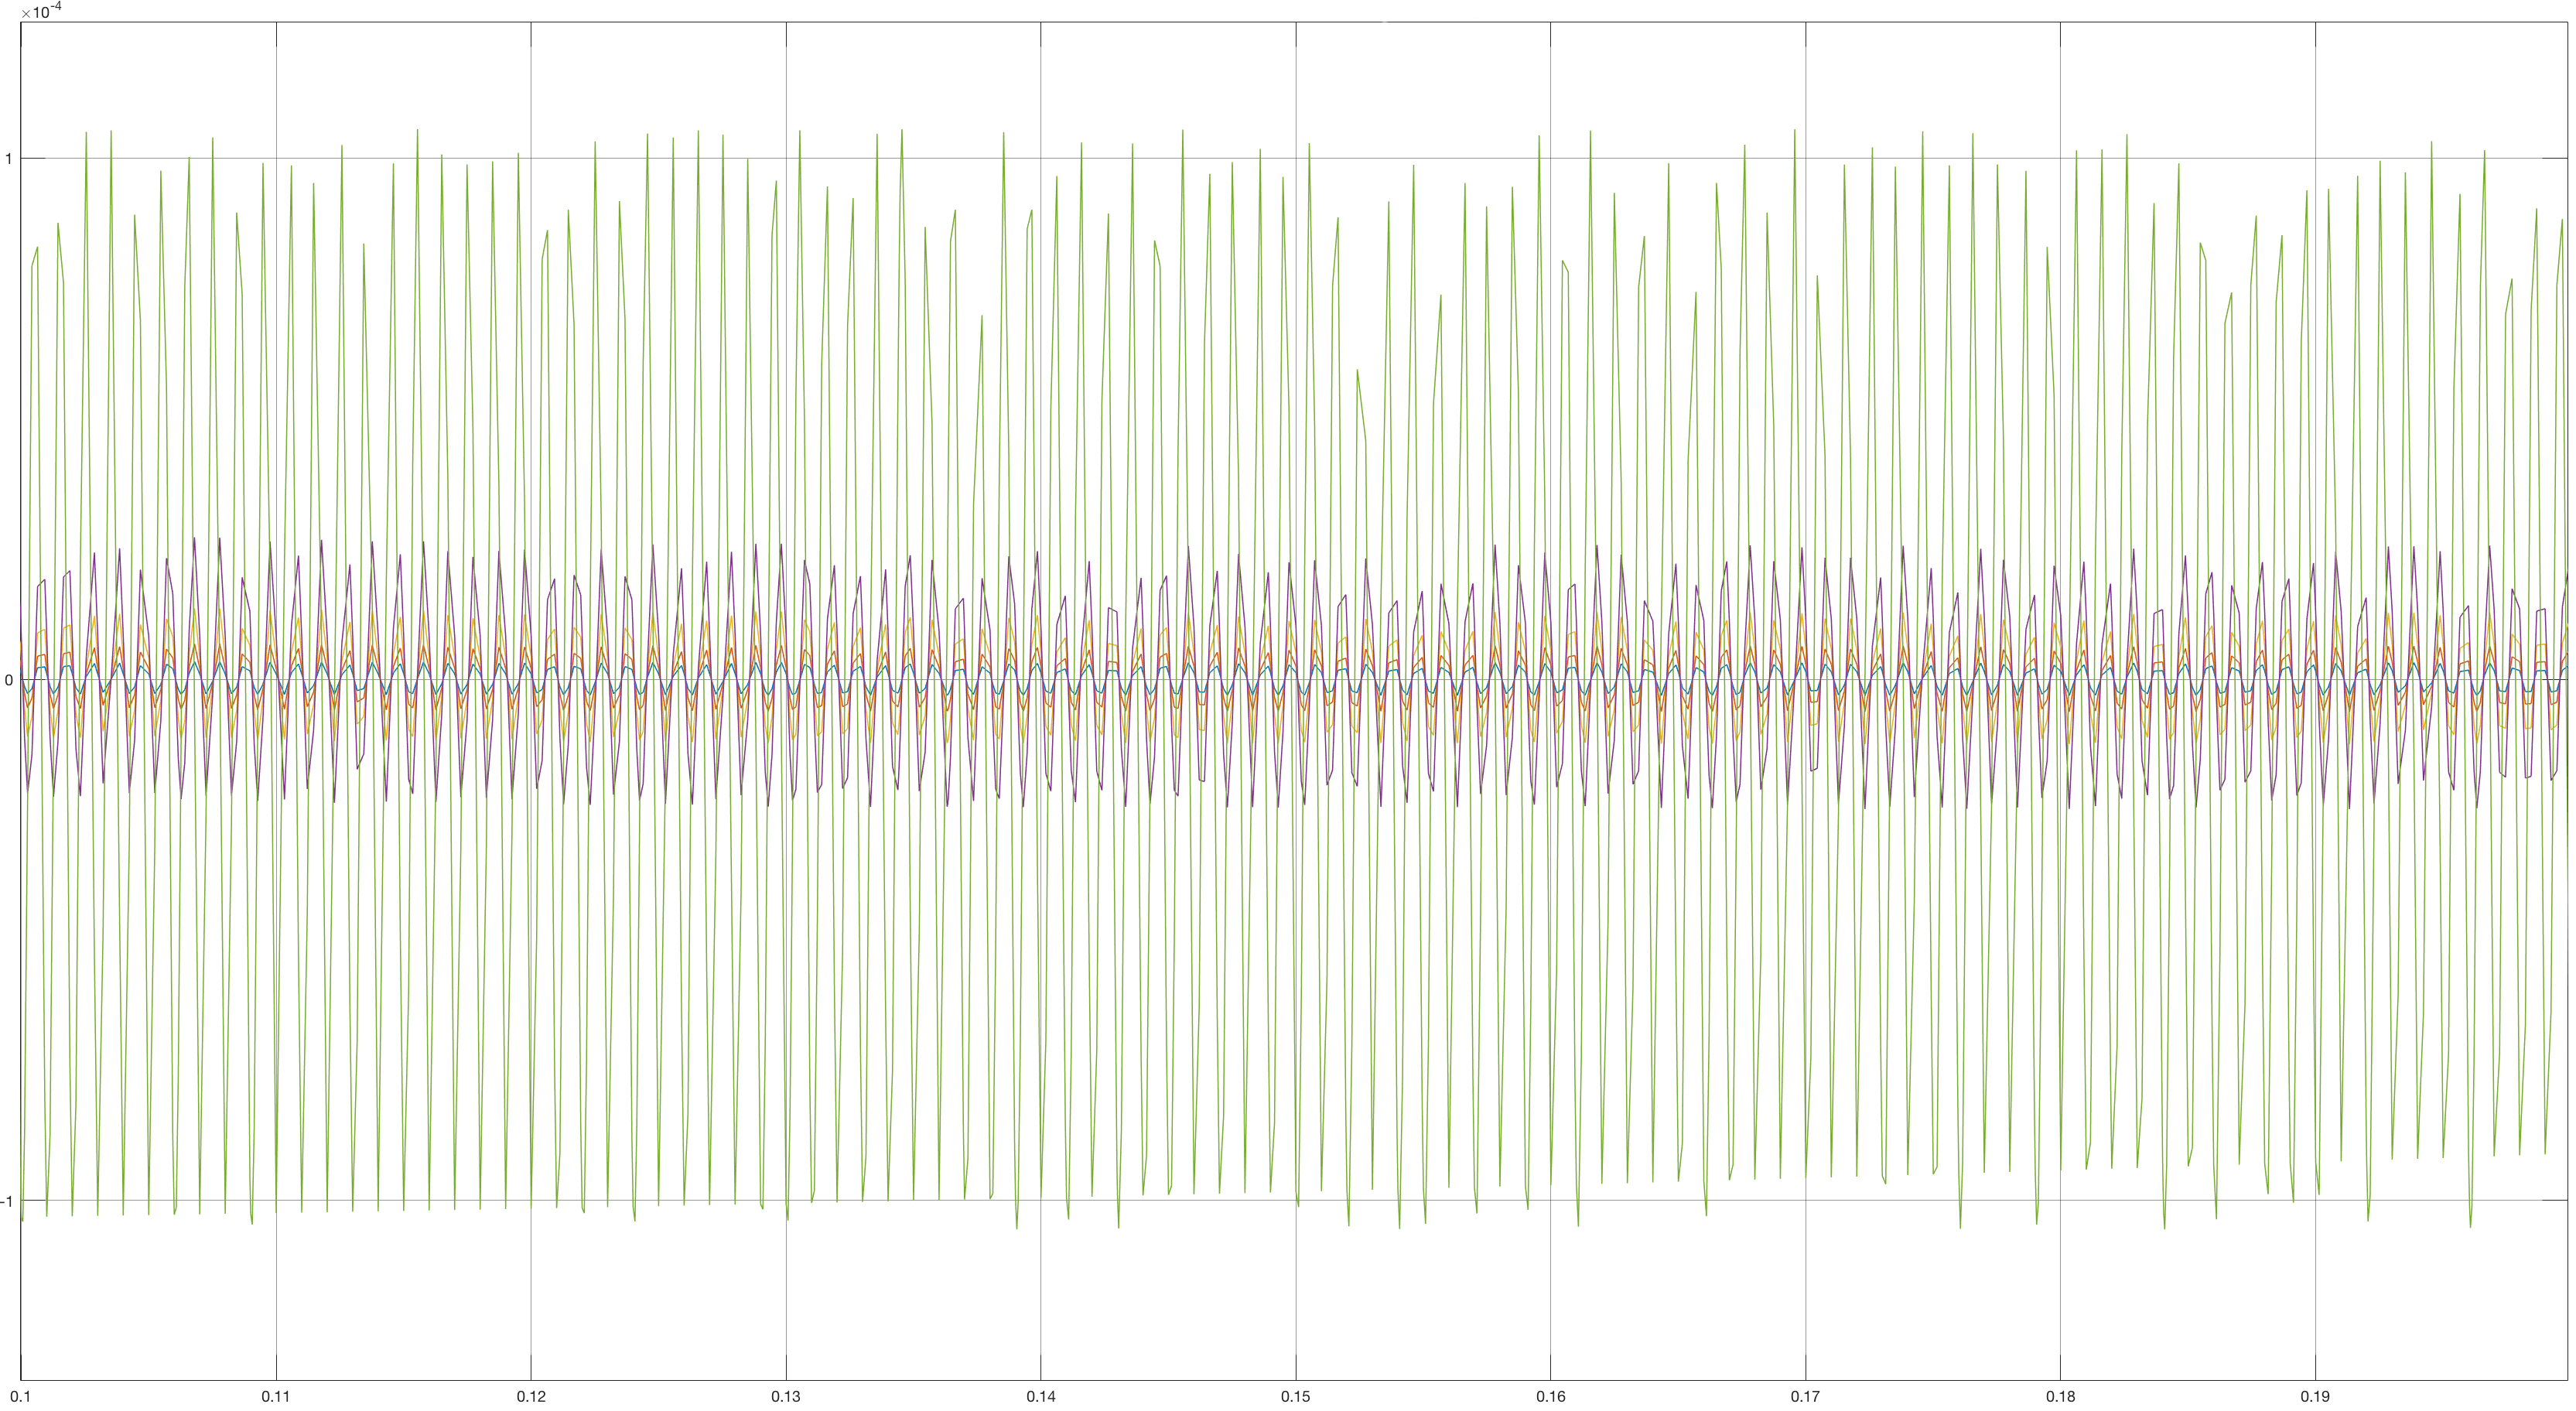
\includegraphics[width=\textwidth, height=0.29\textwidth]{Images/vibr1000Htz}
		\caption{1000 Hz}
		\label{fig:1000Htz}
	\end{subfigure}
\caption{Slave position response to a sinusoidal input with three different frequencies.}
\label{positionResponceFrequencies}
\end{figure}

\newpage

\subsection{Task execution analysis}

\subsubsection*{Simulation setup}

The operator is modeled as spring-damper system ($ K=200.0 \ \text{N/m} $ and $ B=4.0 \ \text{N}\cdot\text{s}/\text{m} $). The master-slave system has arms of length equal to $ 0.1 \text{m} $. 

The environment with which the slave manipulator comes into contact is modeled as:
\begin{itemize}
	\item free motion: the environment has no stiffness but just a small damping $ B_{env}=0.01 \text{N}\cdot\text{s}/\text{m} $;
	\item contact motion: the environment has large stiffness $ K_{env} = 4000.0 \ \text{N/m} $ after a chosen value of displacement.
\end{itemize}

The simulation are exerted with the \textbf{control set 4} ($ K_v = 20.0 \frac{\text{N m}}{\text{rad}} $, $ B_v = 4.4\cdot 10^{-1} \ \frac{\text{N m}}{\text{rad/s}}$, $ J_v = 3\cdot 10^{-4} \ \text{kg m\textsuperscript{2}}$) and are compared with the \textbf{rigid coupling control} ($K_v = 10^{2} \ \frac{\text{N m}}{\text{rad}} $, $B_v = 1.5\cdot 10^{-1} \ \frac{\text{N m}}{\text{rad/s}}$, $J_v =  0 \ \text{kg m\textsuperscript{2}} $).

\subsubsection{Free motion with high frequency input}

At first, we present an execution in free motion. The slave manages to mirror the master which is moved according to a $ 0.11 \ \text{Hz} $ sinusoidal trajectory. Applying both \textsl{rigid coupling control} (fig.\ref{fig:freeRigTot50HR}) and \textsl{virtual compliance control} (fig.\ref{fig:freeSetTot50HR}).
% with almost no task error (without considering the error due to noise disturbances).

The noise of the system is modeled a mixture of white noise and sinusoidal oscillations both at frequency of $50 \ \text{Hz}$ on the slave side.

\begin{figure}[H]
	\begin{subfigure}{1\linewidth}
		\centering
		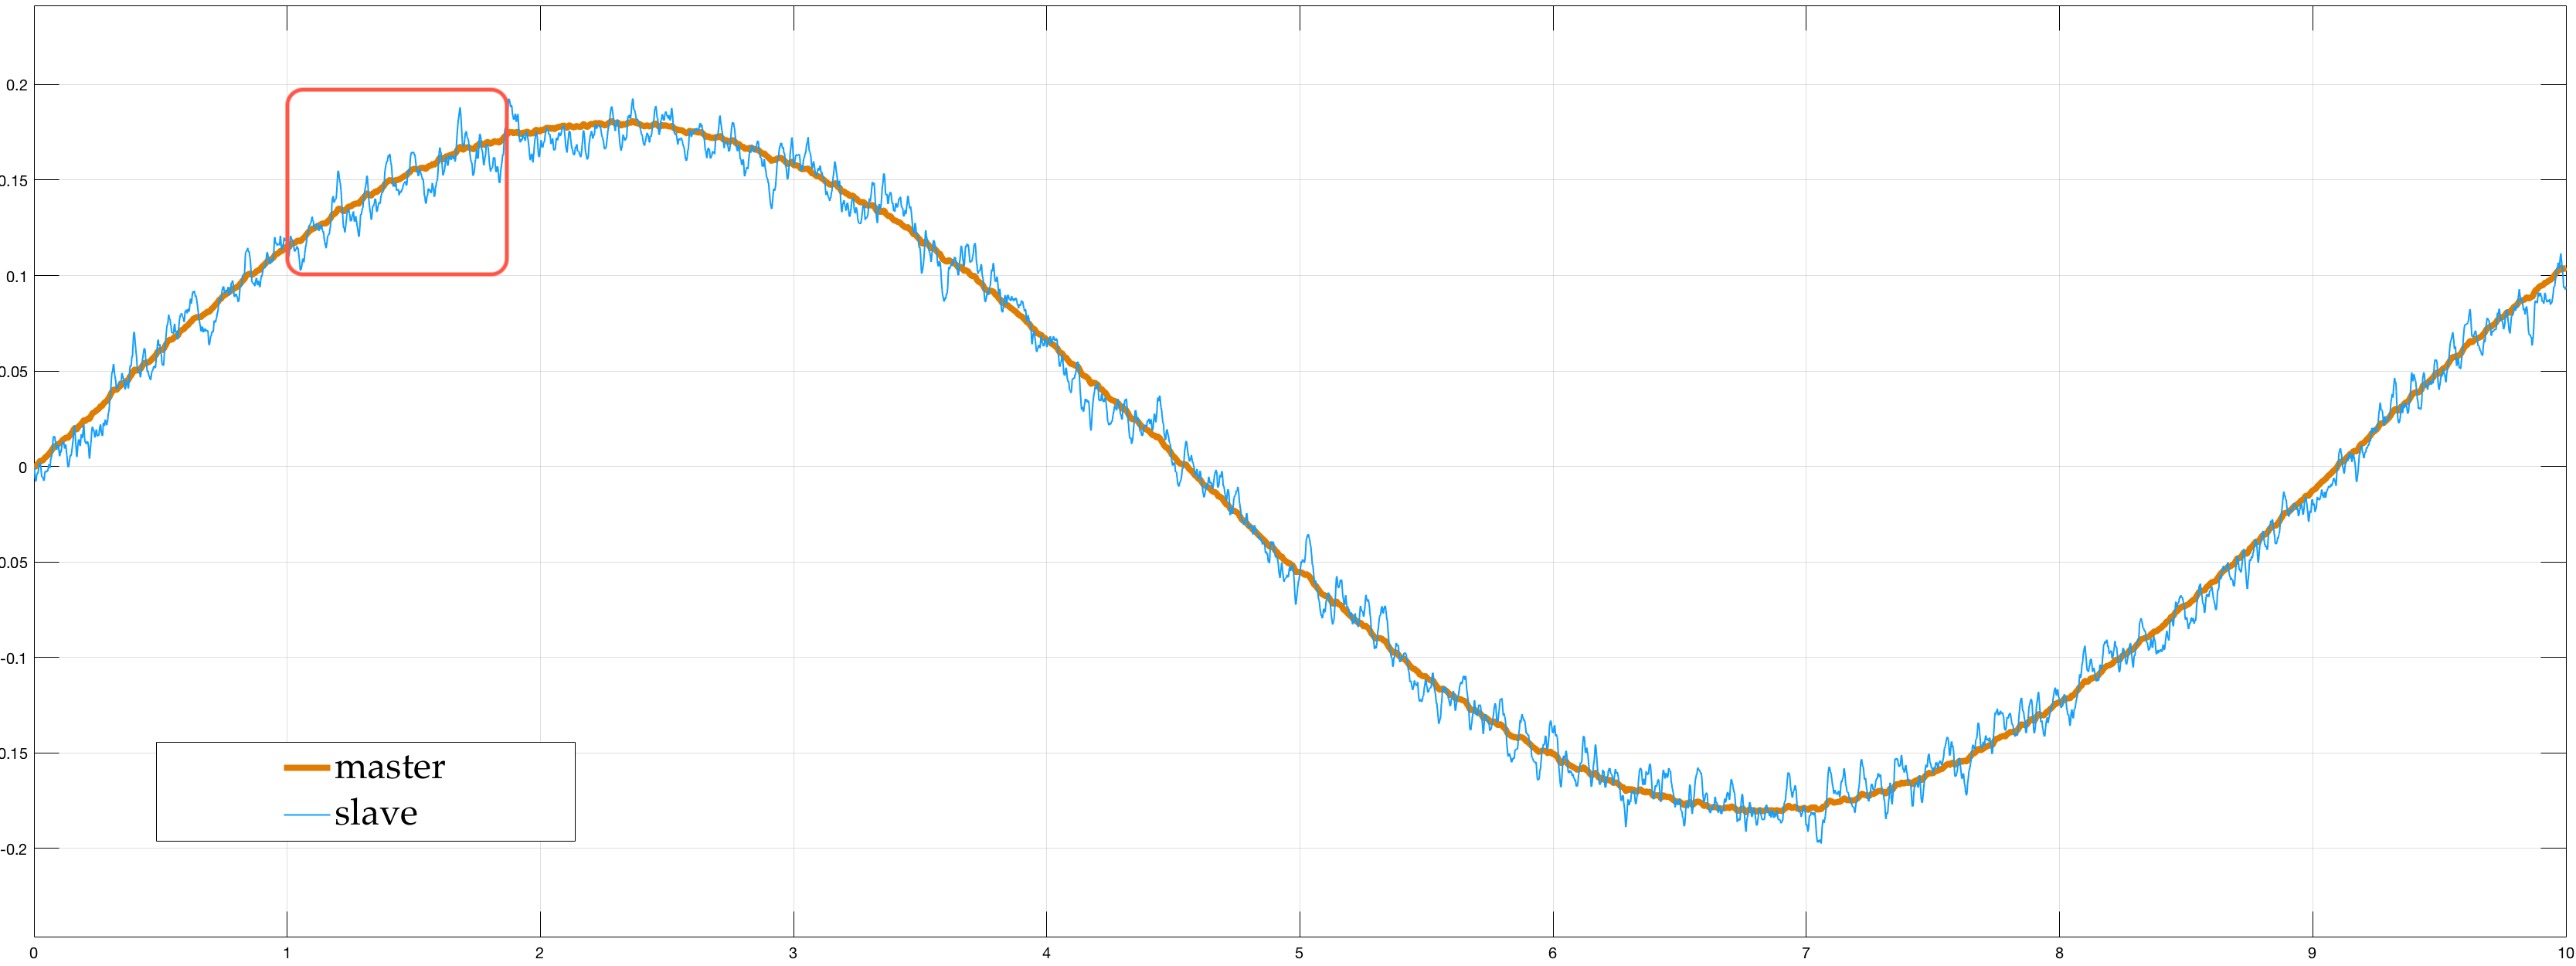
\includegraphics[width=\textwidth, height=0.48\textwidth]{Images/set20freeTot50HtznoiseRect}
		\caption{Positions of the master-slave system in free motion - virtual compliance control.}
		\label{fig:freeSetTot50HR}
	\end{subfigure}	
\end{figure}
\begin{figure}\ContinuedFloat
	\begin{subfigure}{1\linewidth}
		\centering
		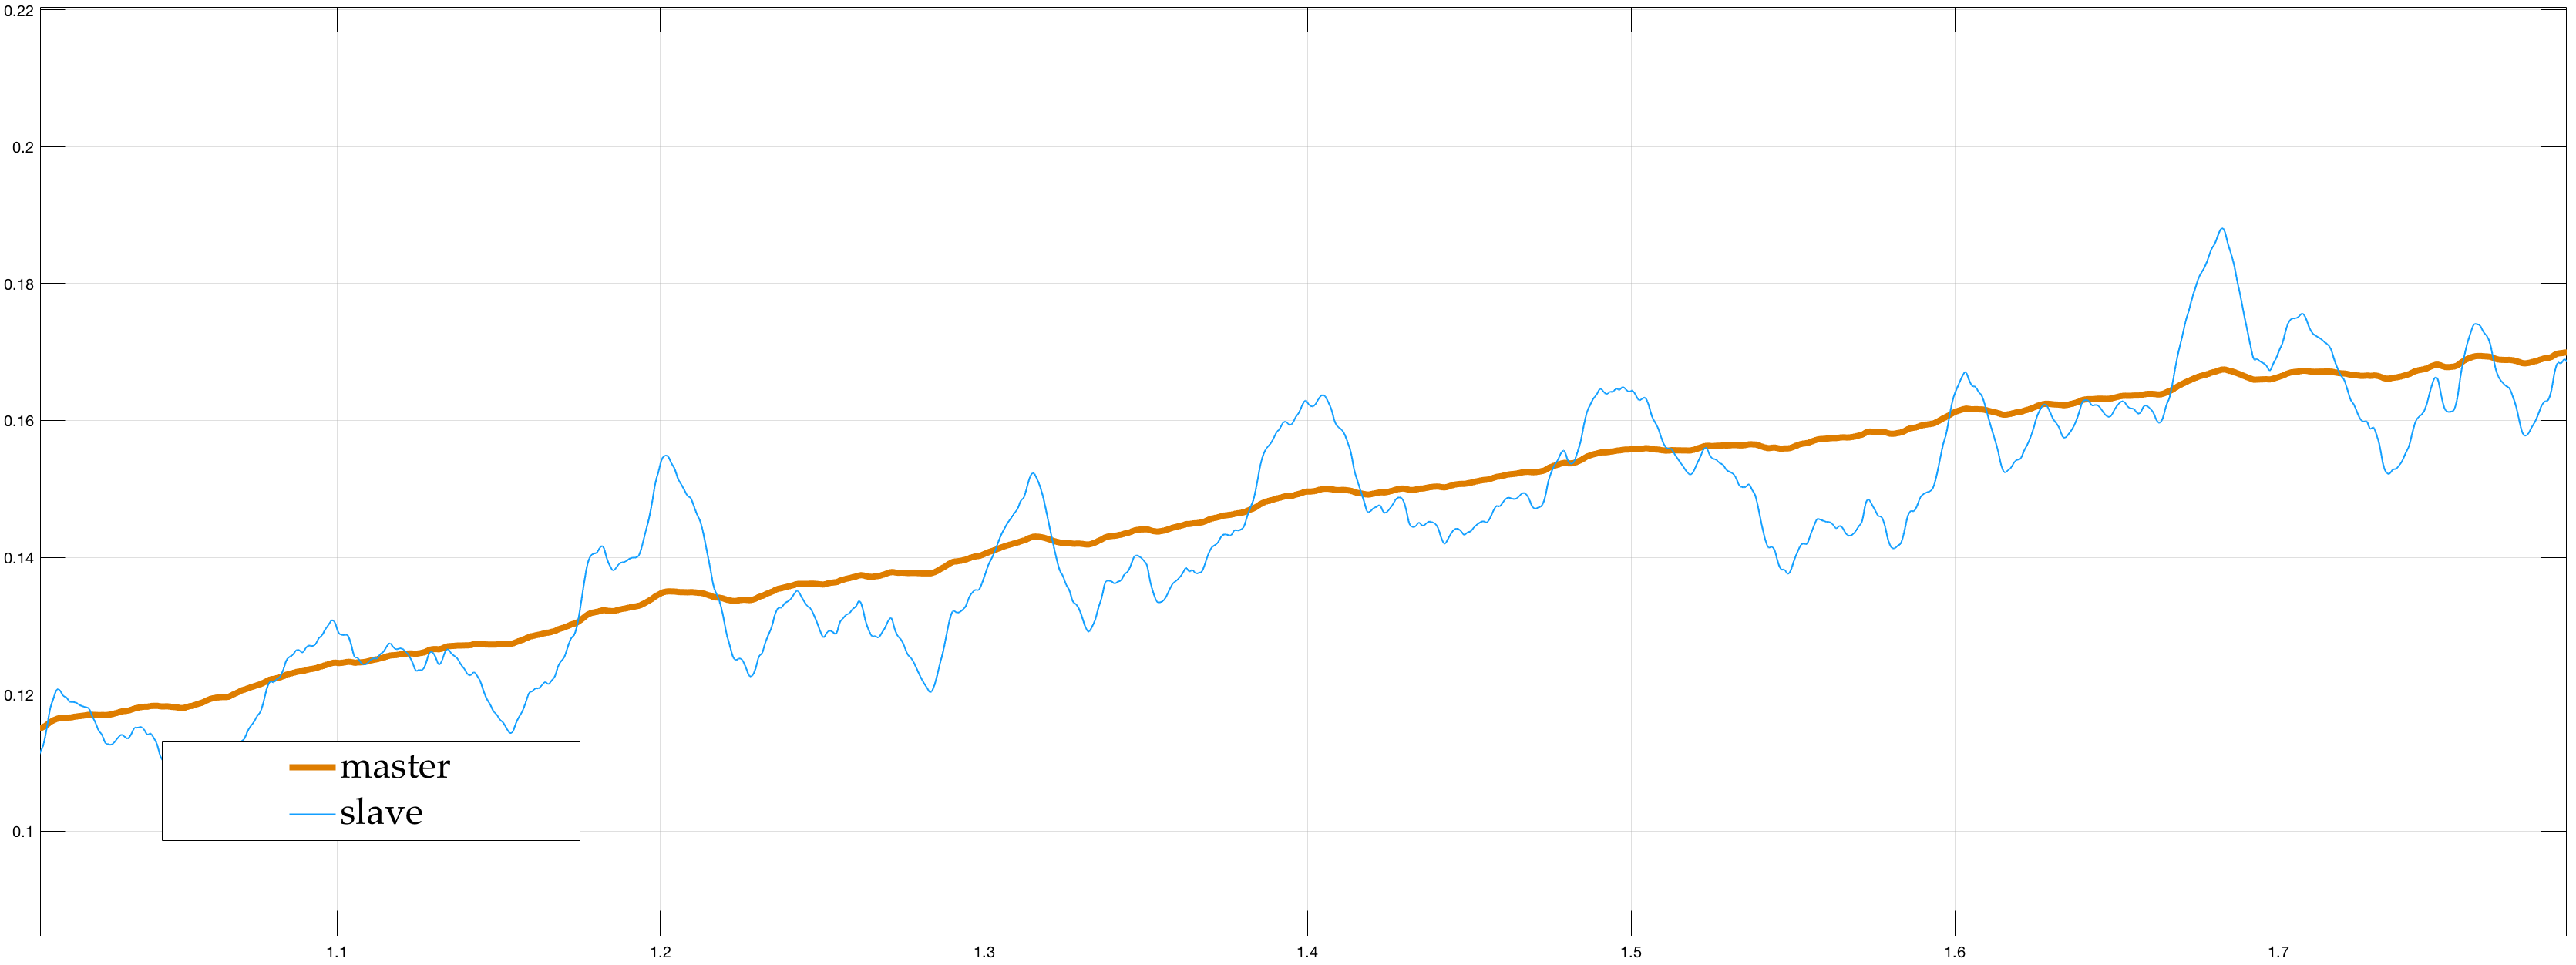
\includegraphics[width=\textwidth, height=0.48\textwidth]{Images/set20freePart50Htznoise}
		\caption{Detail describing the highlighted area in fig.\ref{fig:freeSetTot50HR}}
		\label{fig:freeSetPar50HR}
	\end{subfigure}	
	\caption{\textbf{High} frequency disturbances response - virtual compliance control.}
\end{figure}

\begin{figure}[H]
	\begin{subfigure}{1\linewidth}
		\centering
		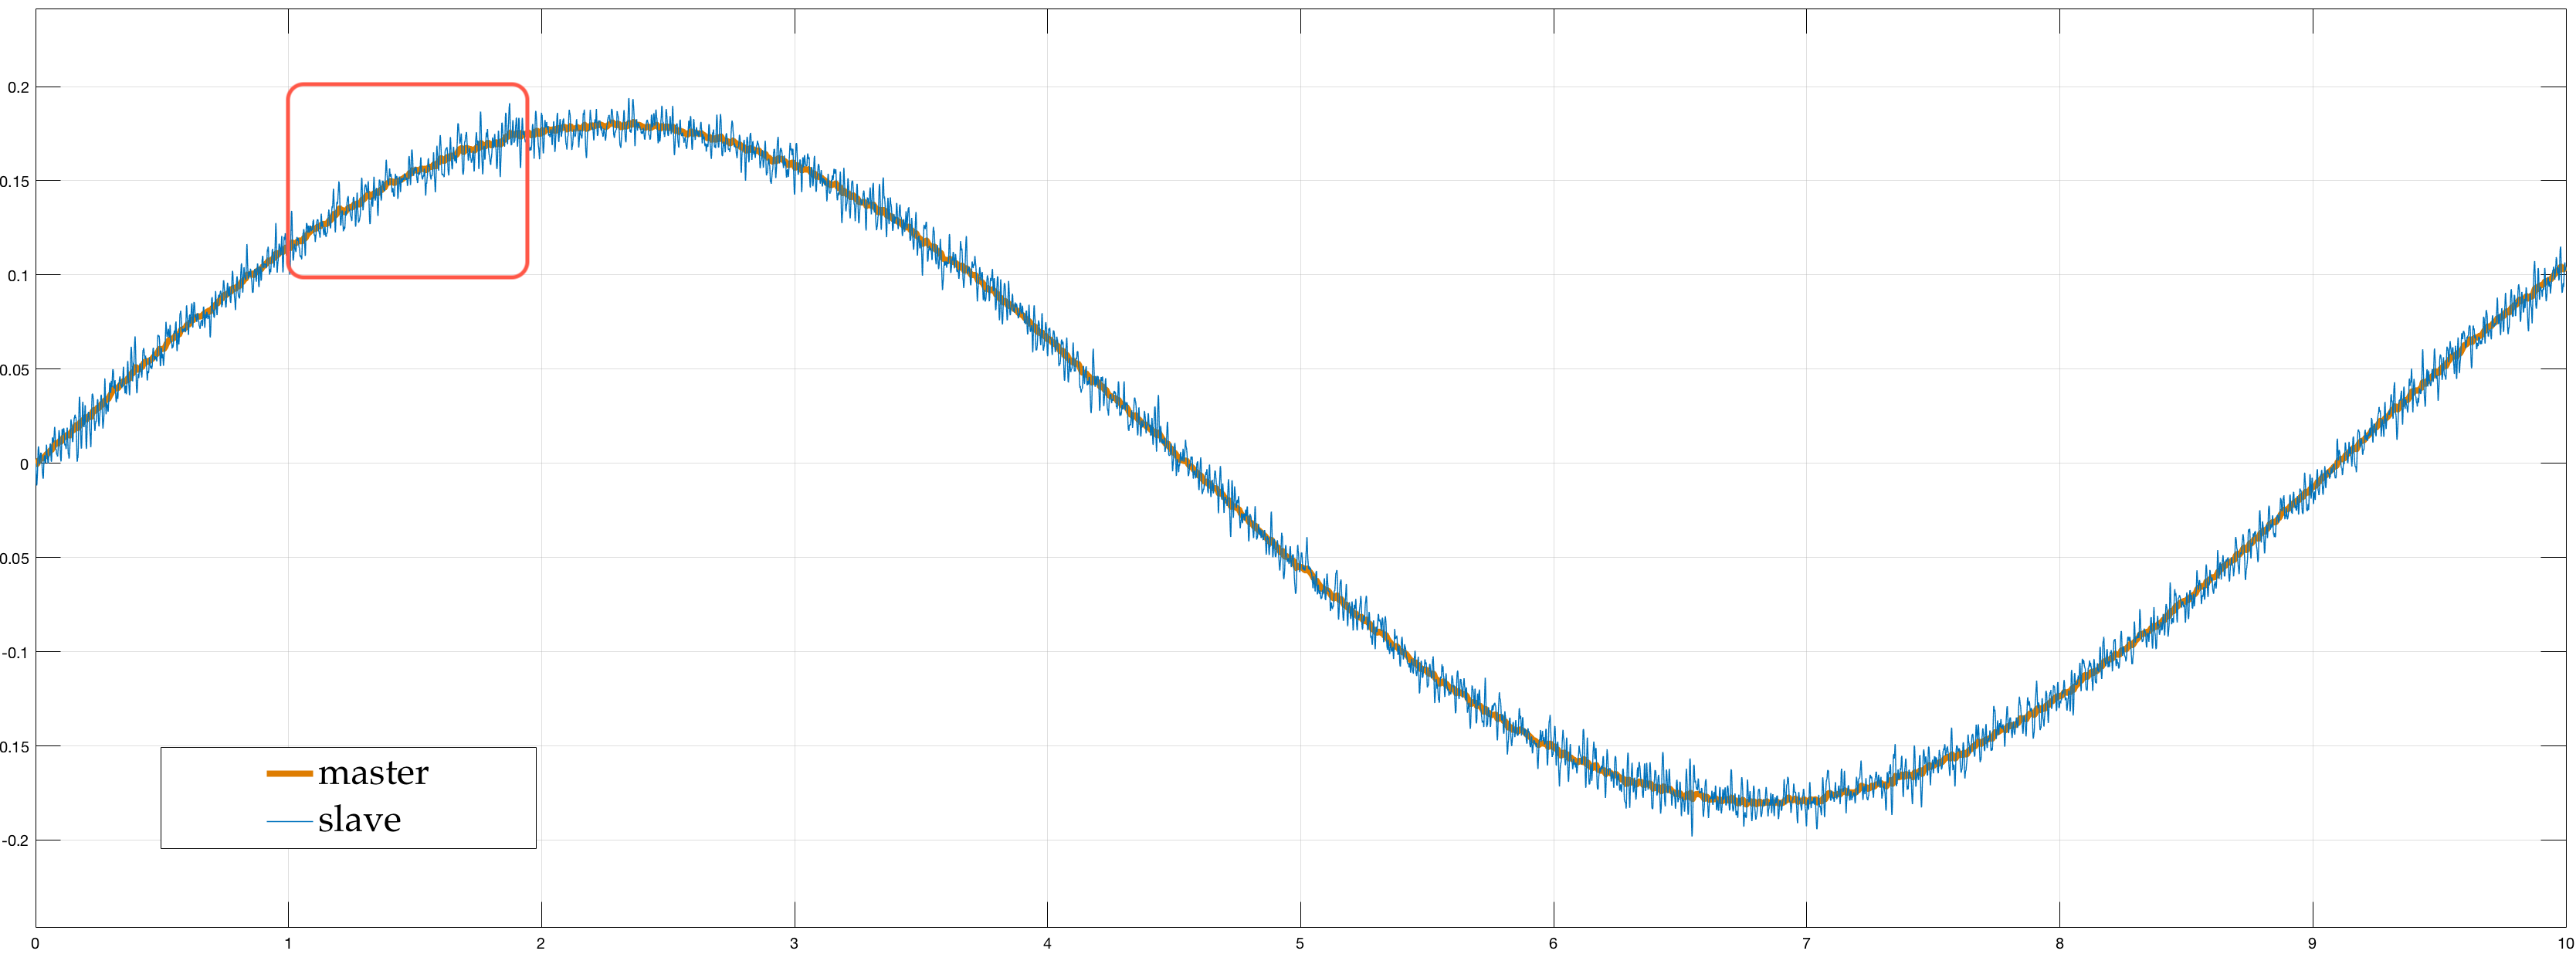
\includegraphics[width=\textwidth, height=0.48\textwidth]{Images/rCoupFreeTot50htznoiseRect}
		\caption{Positions of the master-slave system in free motion - rigid coupling control.}
		\label{fig:freeRigTot50HR}
	\end{subfigure}
\end{figure}
\begin{figure}\ContinuedFloat
	\begin{subfigure}{1\linewidth}
		\centering
		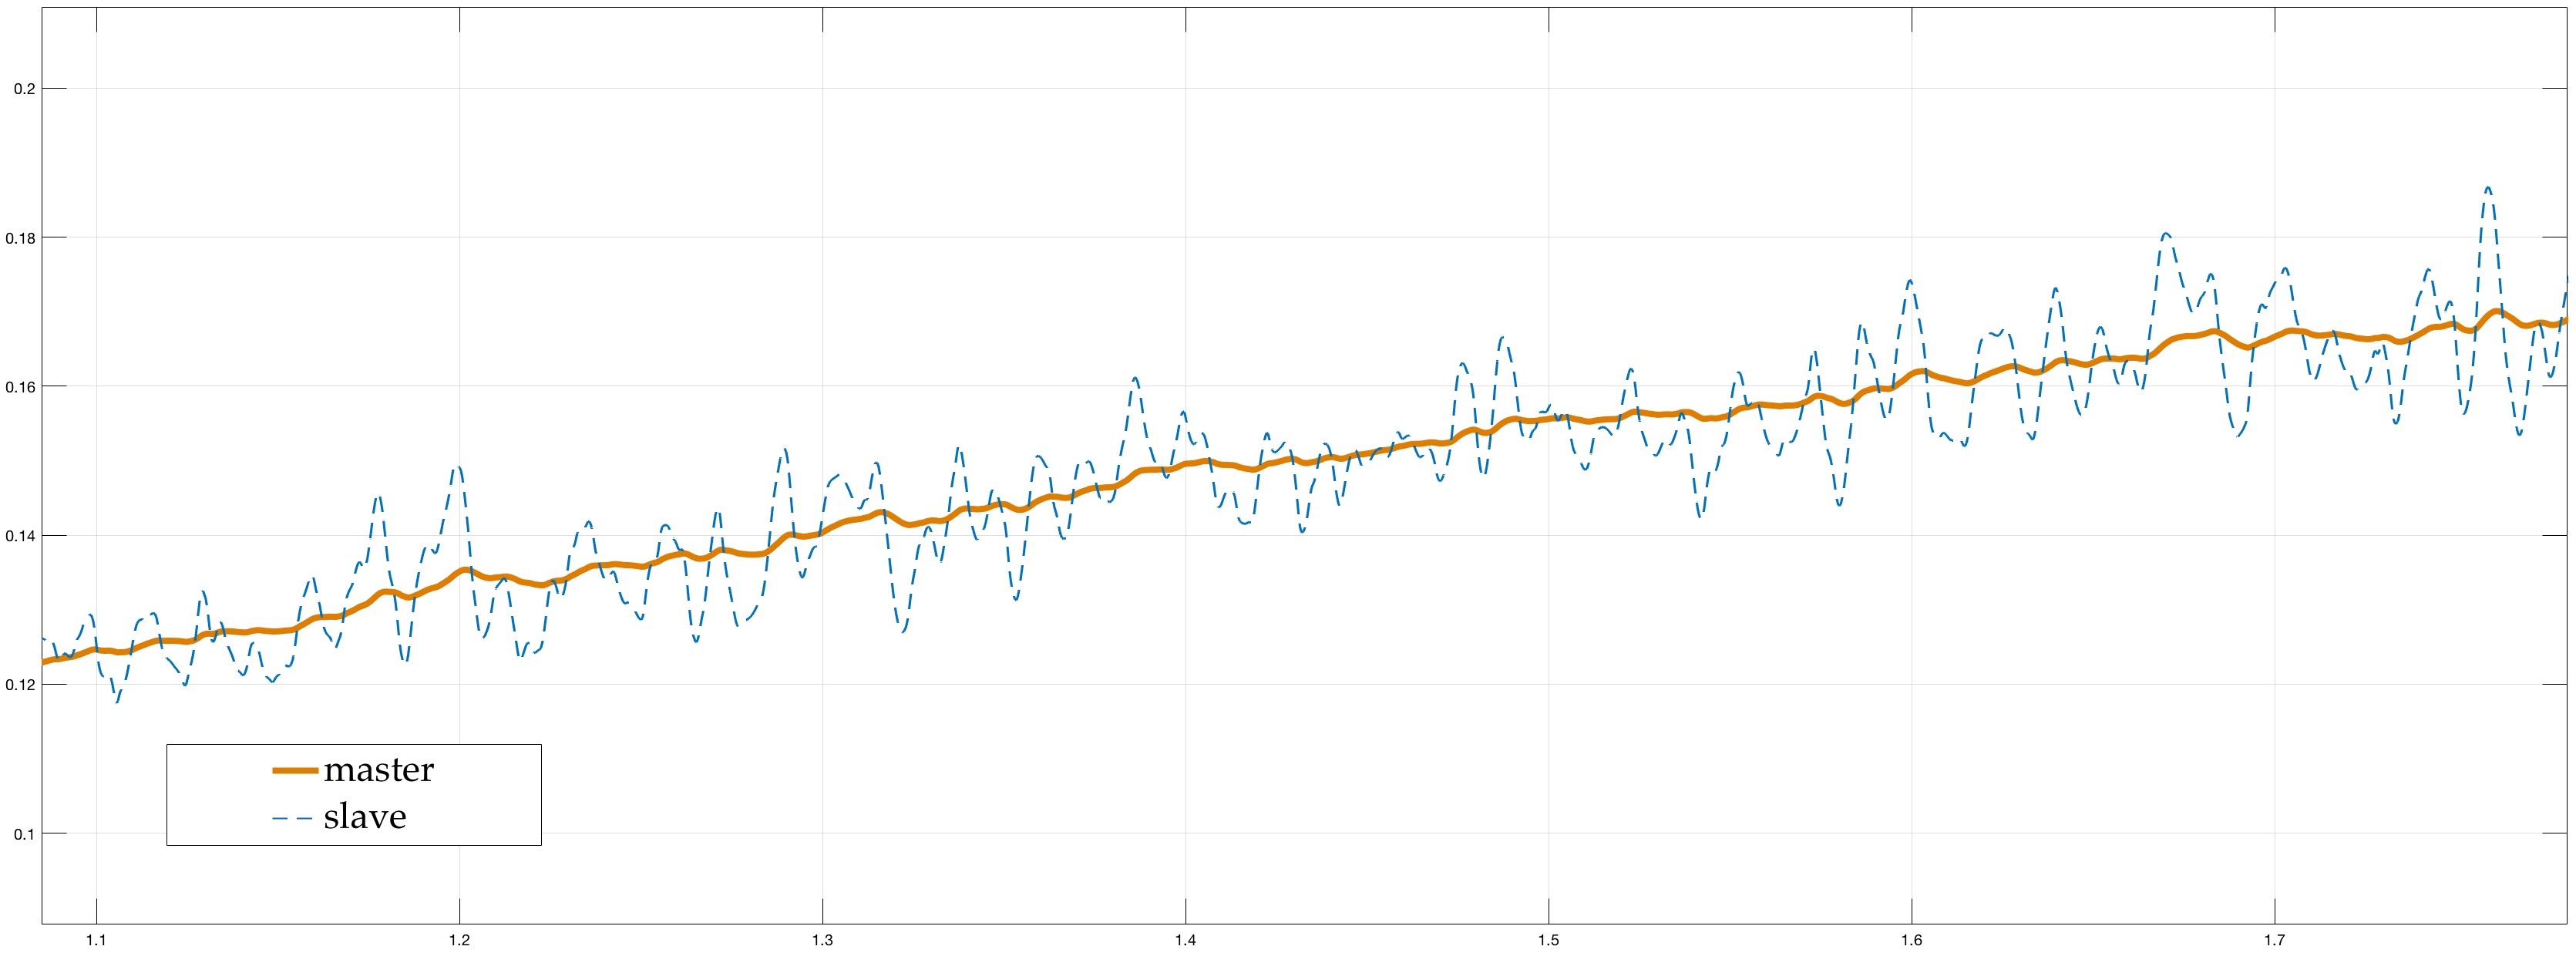
\includegraphics[width=\textwidth, height=0.48\textwidth]{Images/rCoupFree50htznoise}
		\caption{Detail describing the highlighted area in fig.\ref{fig:freeRigTot50HR}.}
		\label{fig:freeRigPar50HR}
	\end{subfigure}	
  \caption{\textbf{High} frequency disturbances response - rigid coupling control.}
\end{figure}

%This kind of disturbance should be damped, and in fact, using \textsl{virtual compliance} (fig.\ref{fig:freeRigPar50HR}) the profile of the angle is smoother than in \textsl{rigid coupling} (fig.\ref{fig:freeRigPar50HR}).

A comparison between the fig.\ref{fig:freeRigPar50HR} and the fig.\ref{fig:freeSetPar50HR} shows how is the slave response under the two different type of controllers: the response is slower using the virtual compliance control respect to the rigid coupling control. By consequence, the operator "feels" less disturbances. 

\subsubsection{Free motion with low frequency input}

Comparatively, two other simulations have been undertaken that share the same
conditions of the previous ones. Here the input frequency is lowered to $20 \ \text{Hz}$.

It is desired for this type of inputs to be detectable, and hence, they should be preserved. 
%This kind of input are usually a similar to the input of the control
%actuators, so it should be preserved, namely it shouldn't be affected by the
%proposed filtering.

\begin{figure}[H]
	\begin{subfigure}{1\linewidth}
		\centering
		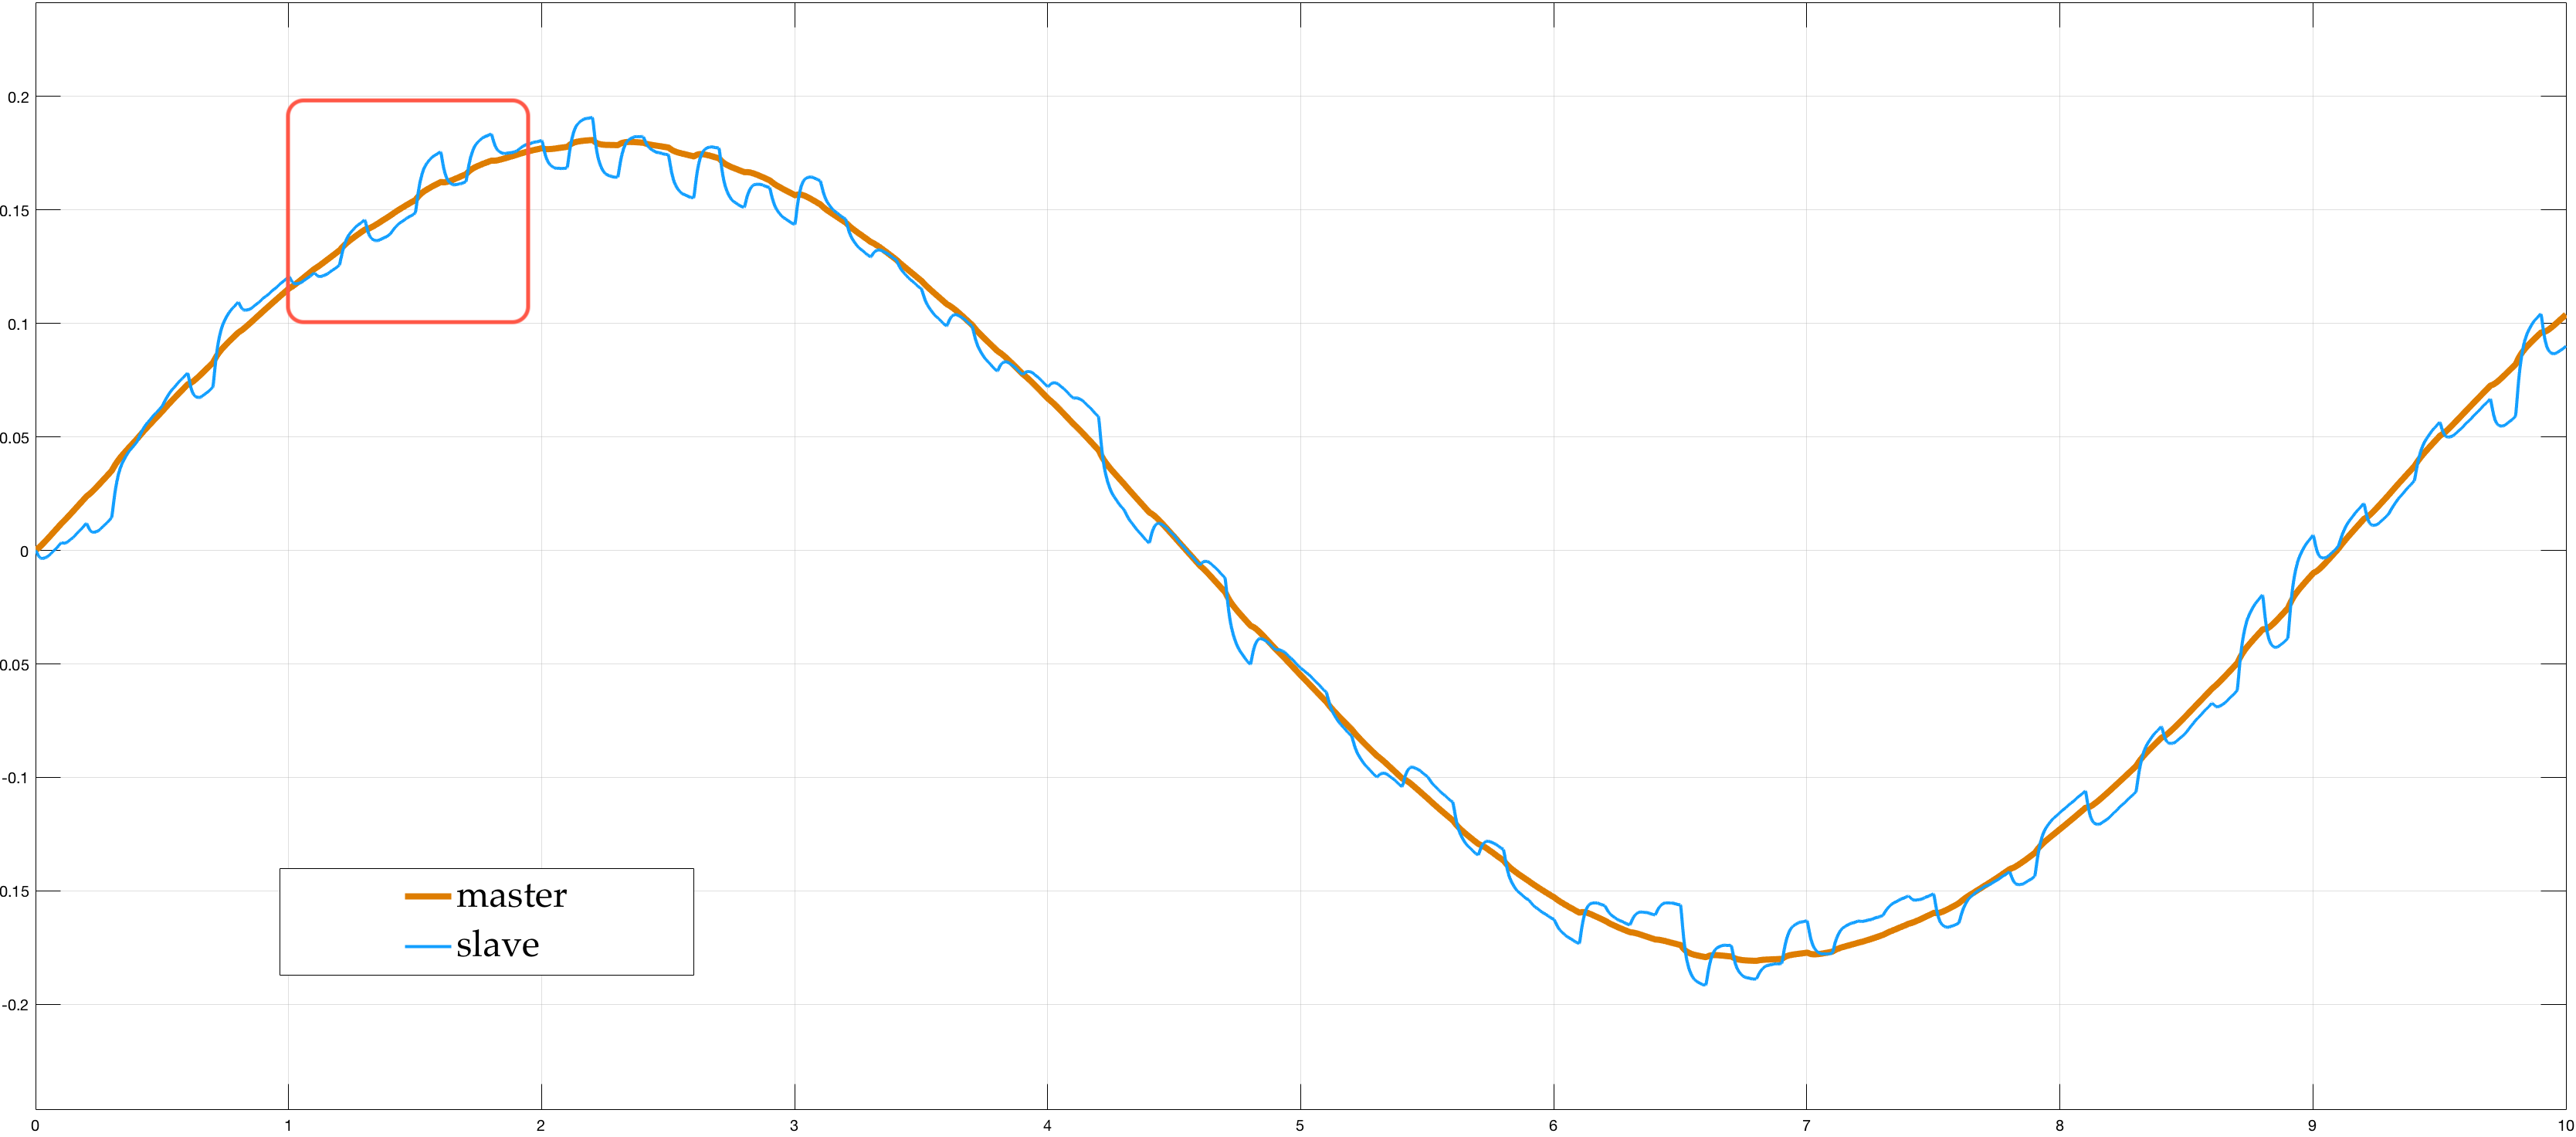
\includegraphics[width=\textwidth, height=0.48\textwidth]{Images/freeSet20Tot20HtznoiseRect}
		\caption{Positions of the master-slave system in free motion - virtual compliance control.}
		\label{fig:freeSetTot20HR}
	\end{subfigure}
\end{figure}
\begin{figure}\ContinuedFloat
	\begin{subfigure}{1\linewidth}
		\centering
		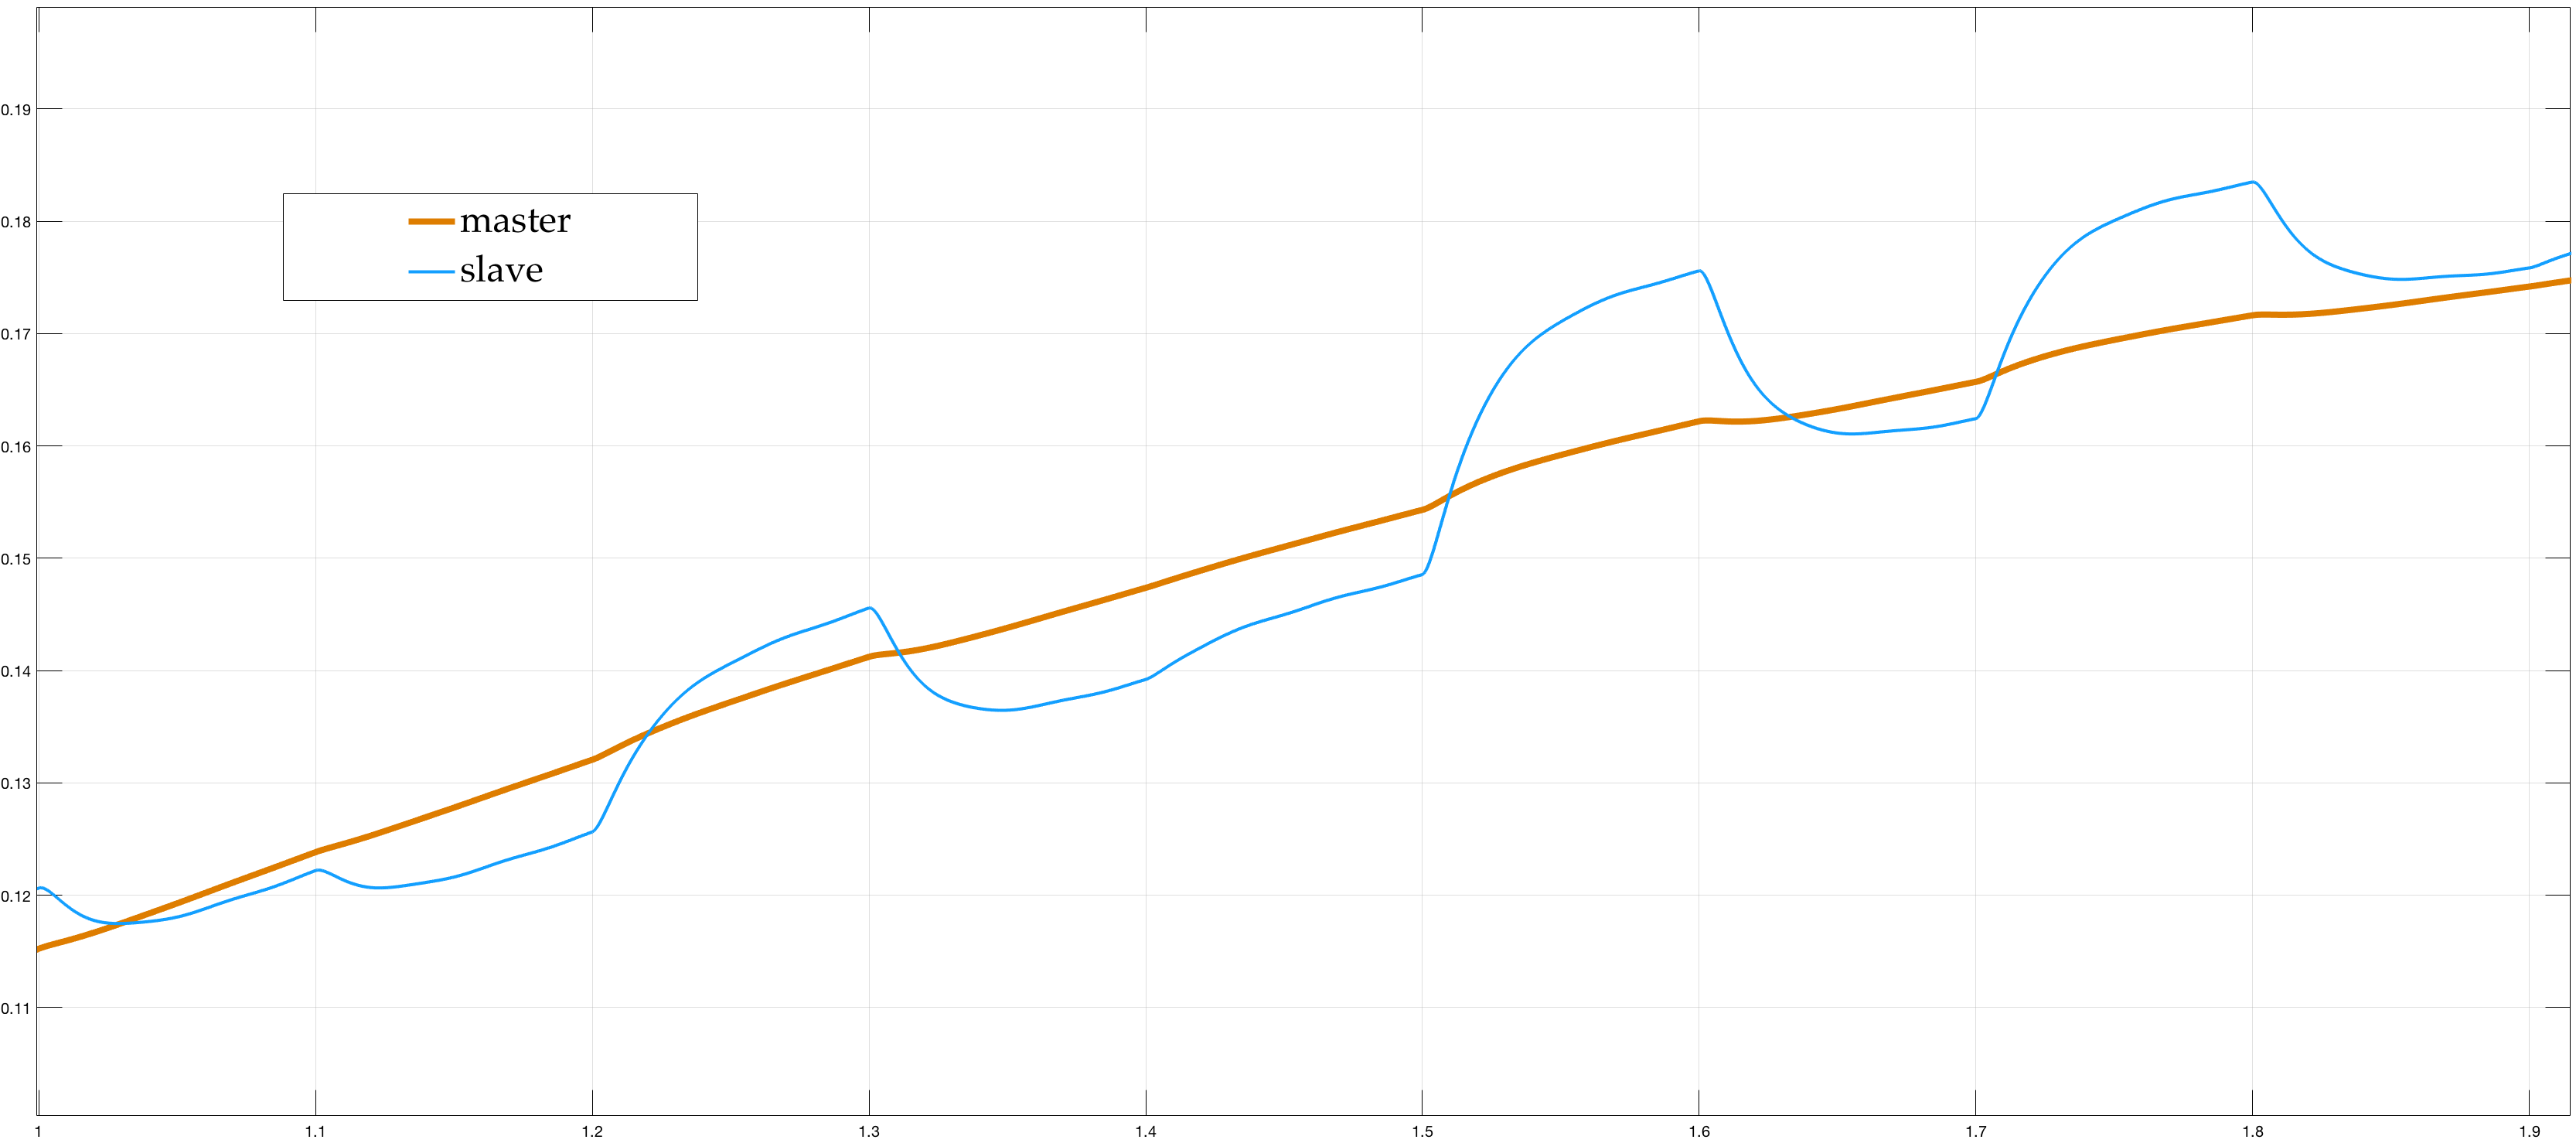
\includegraphics[width=\textwidth, height=0.48\textwidth]{Images/freeSet20Part20Htznoise}
		\caption{Detail describing the highlighted area in fig.\ref{fig:freeSetTot20HR}}
		\label{fig:freeSetPar20HR}
	\end{subfigure}	
	\caption{\textbf{Low} frequency disturbances response - virtual compliance control.}
\end{figure}

\begin{figure}[H]
	\begin{subfigure}{1\linewidth}
		\centering
		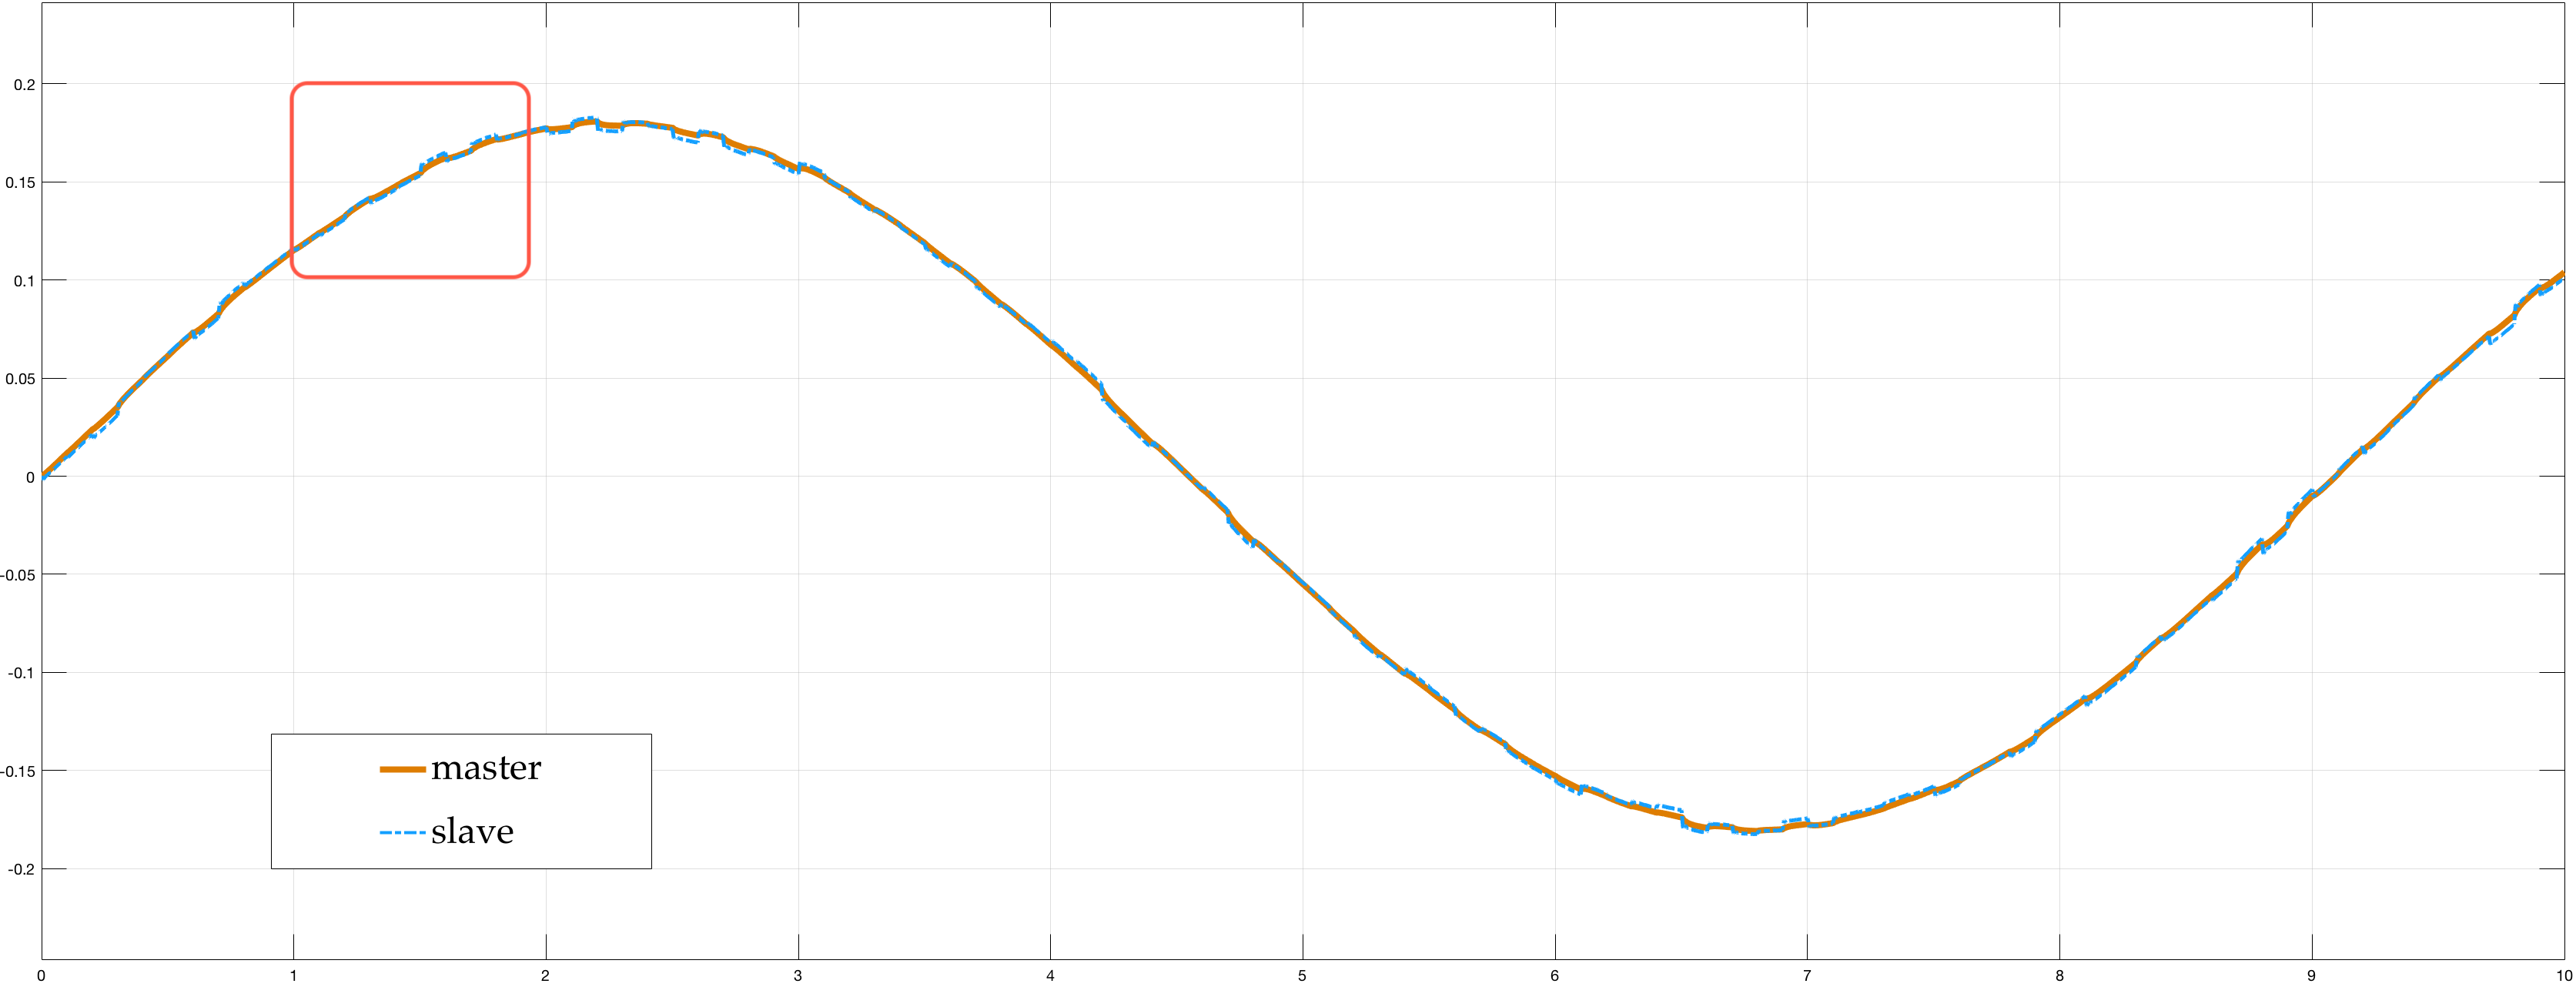
\includegraphics[width=\textwidth, height=0.48\textwidth]{Images/freerigidTot20HtznoiseRect}
		\caption{Positions of the master-slave system in free motion - rigid coupling control.}
		\label{fig:freeRigTot20HR}
	\end{subfigure}	
\end{figure}
\begin{figure}\ContinuedFloat
	\begin{subfigure}{1\linewidth}
		\centering
		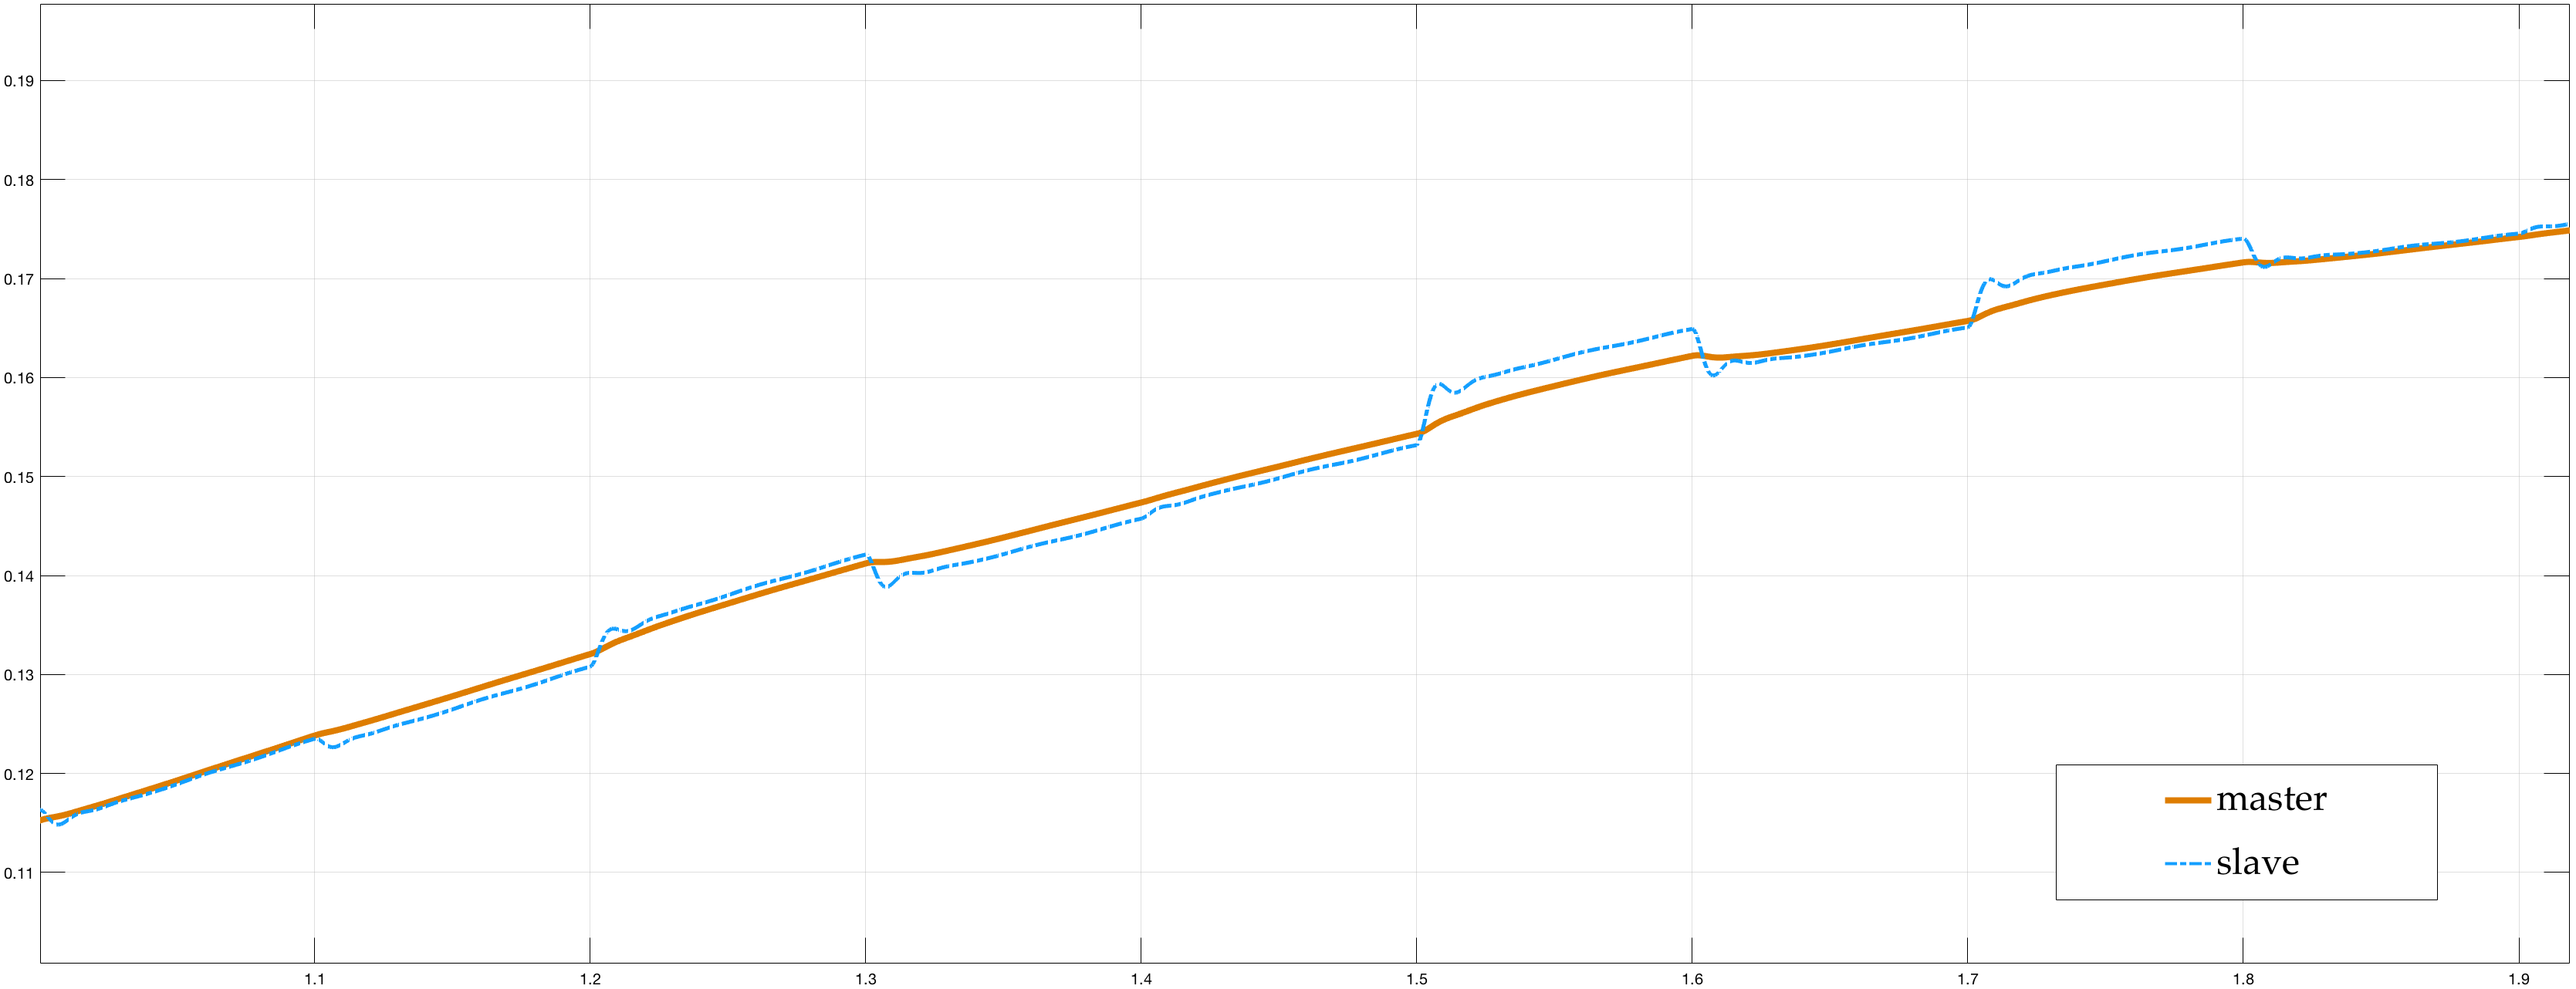
\includegraphics[width=\textwidth, height=0.48\textwidth]{Images/freerigidPart20Htznoise}
		\caption{Detail describing the highlighted area in fig.\ref{fig:freeRigTot20HR}}
		\label{fig:freeRigPar20HR}
	\end{subfigure}	
 \caption{\textbf{Low} frequency disturbances response - rigid coupling control.}
\end{figure}

This phenomenon shows up in fig.\ref{fig:freeRigPar20HR} and fig.\ref{fig:freeSetPar20HR}. In fact, if compared, the two profiles confirm that \textsl{rigid coupling control} cancel out most of the useful information from the signal.

On the other side \textsl{virtual compliance control} saves the signal information.
%which is extremely important from a control perspective.

\subsubsection{Contact motion}

%In this section the proposed simulations hold the same reference trajectory for
%master than the simulations in free motion. 

In this section the reference trajectory for master is equal to the one used for the simulations in free motion.

%But, in addiction, after that the slave would trespass a certain angle value
%there would be a contact with the environment, this wouldn't allow a perfect
%tracking by the slave.

The slave, overcoming a certain angle value, is in contact with the environment. This will not allow a perfect tracking by the slave.

The comparison between \textsl{virtual compliance control} and \textsl{rigid coupling control} in presence of a contact with the environment can be deduced by the
differences in \textbf{magnitude} of the arrows drawn in the fig.\ref{fig:contact_virtual} and fig.\ref{fig:contact_rigid}.

\begin{figure}[H]
	\begin{subfigure}{1\linewidth}
		\centering
		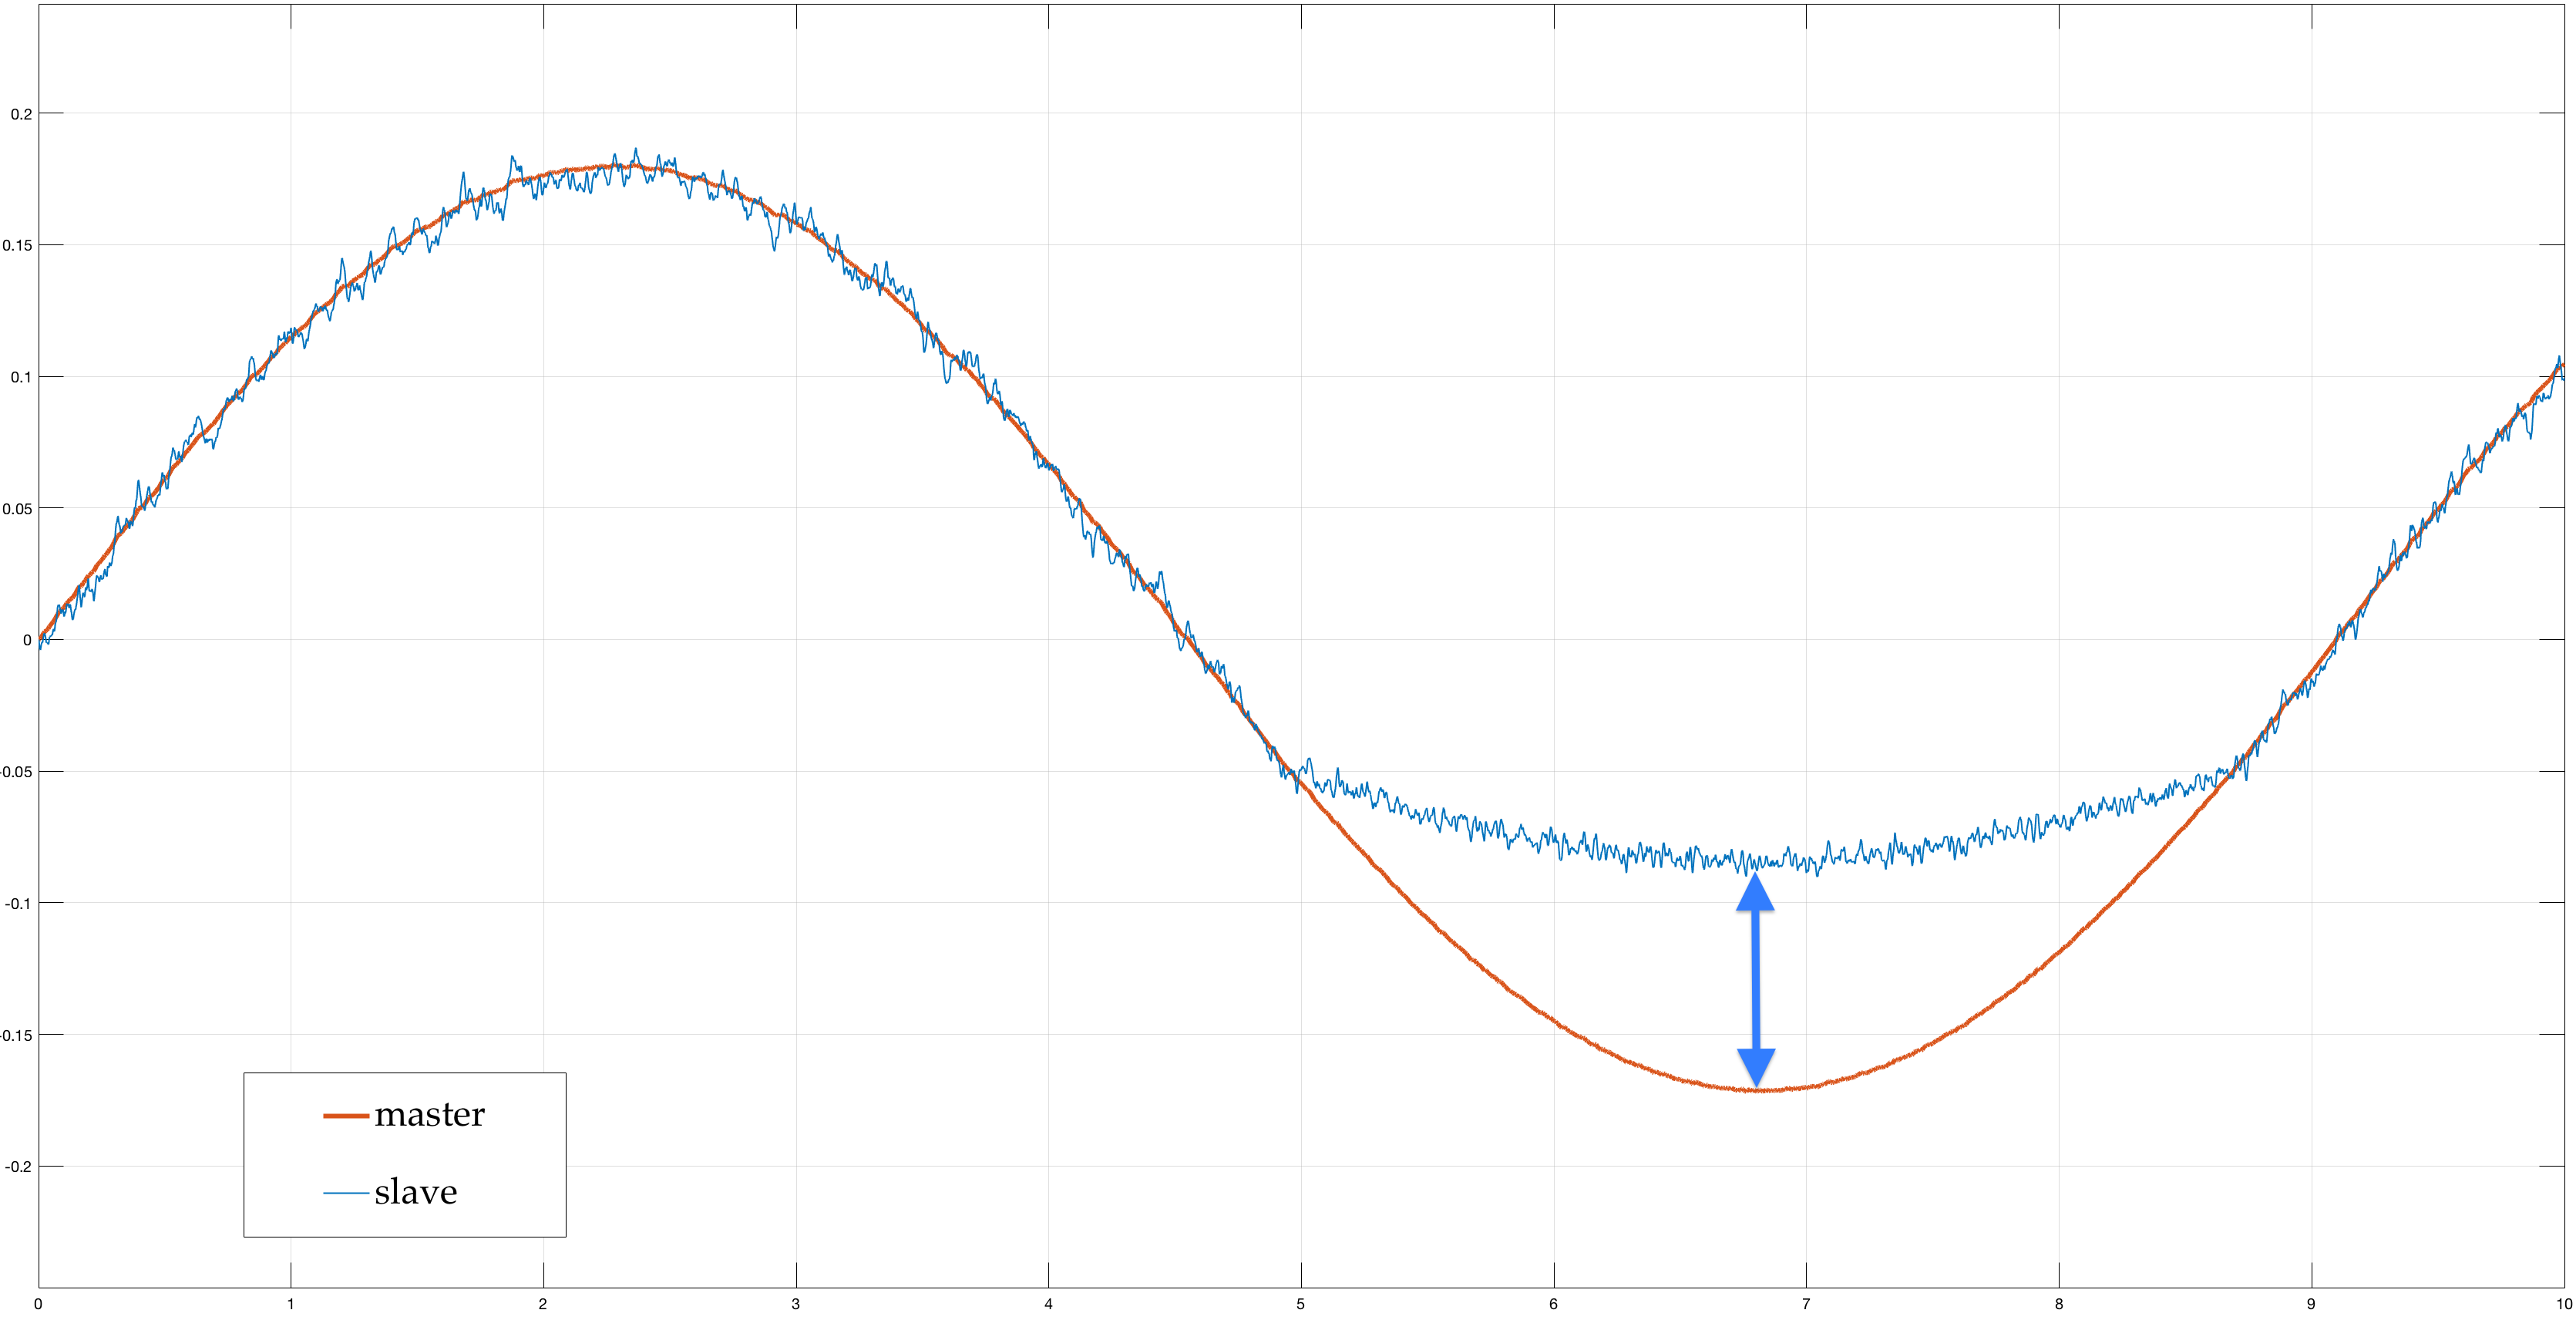
\includegraphics[width=\textwidth, height=0.45\textwidth]{Images/setPointContactReacPosArrow}
		\caption{Position assumed during trajectory tracking.}
		\label{fig:ContactSetPos}
	\end{subfigure}	
\end{figure}
\begin{figure}[H]\ContinuedFloat
	\begin{subfigure}{1\linewidth}
		\centering
		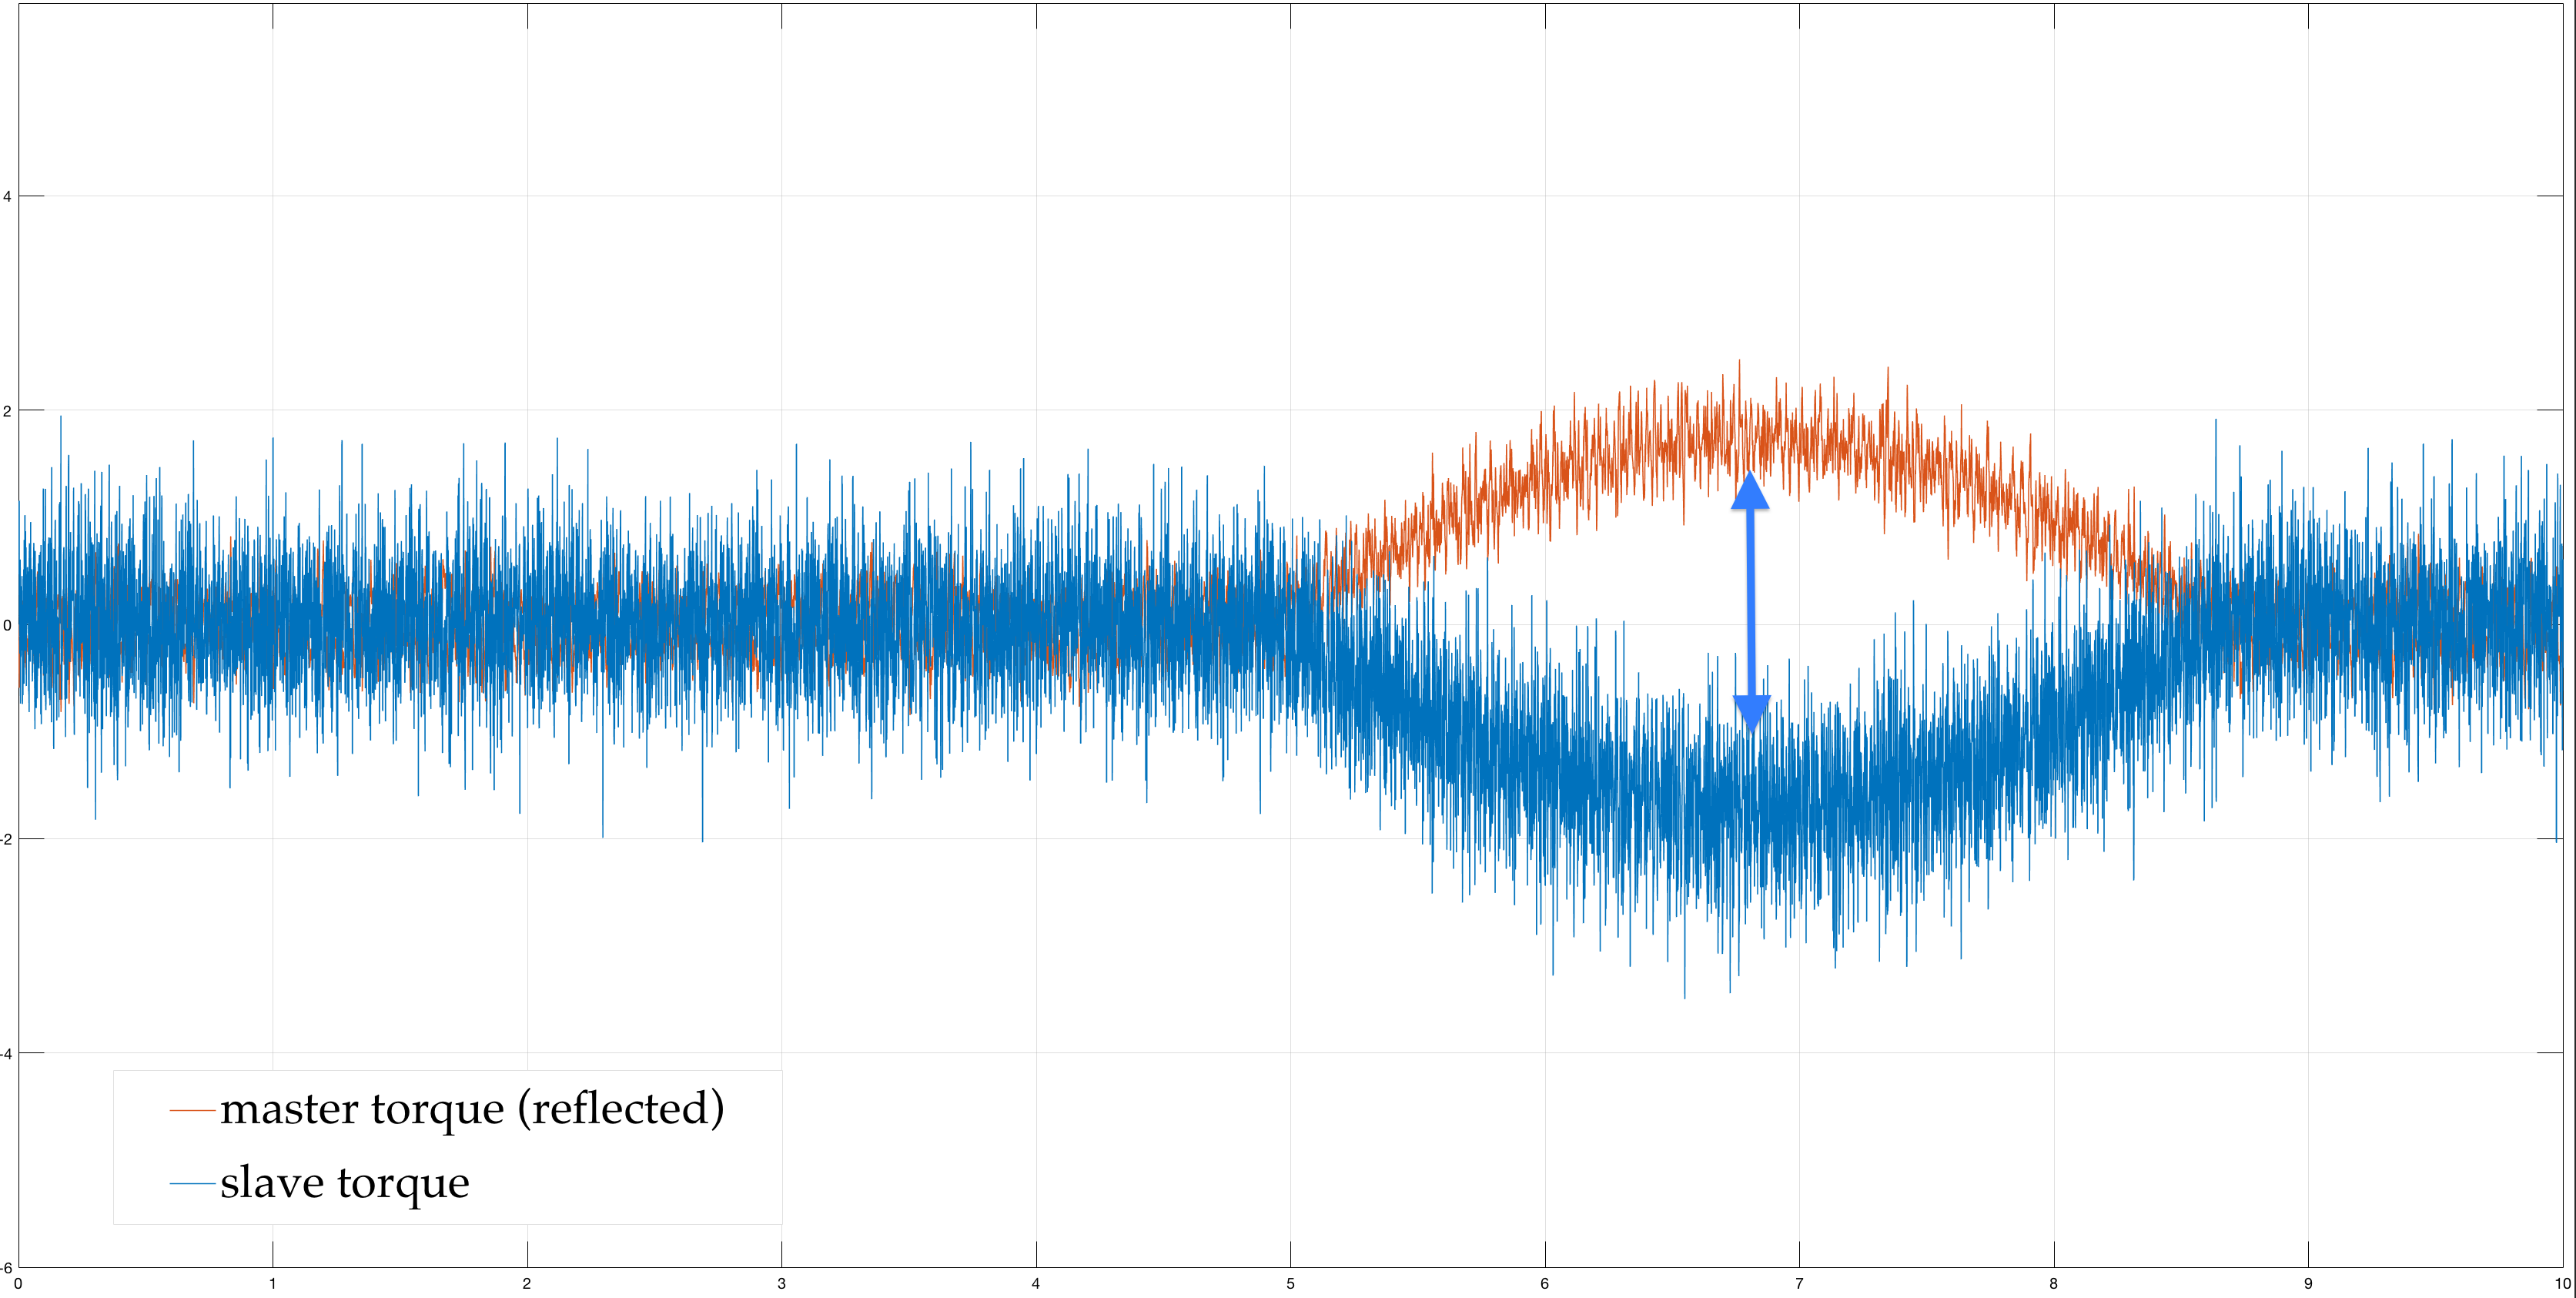
\includegraphics[width=\textwidth, height=0.45\textwidth]{Images/setPointContactReacTorArrow}
		\caption{Torques exerted over time.}
		\label{fig:ContactSetTor}
	\end{subfigure}	
 \caption{Contact motion simulation - virtual compliance control.}
 \label{fig:contact_virtual}
\end{figure}

%Concerning the position of slave with the respect of master the
%fig.\ref{fig:ContactSetPos} portraits a worse performance in trajectory error
%when in contact behaving in \textsl{virtual compliance} than behaving in
%\textsl{rigid coupling} (fig.\ref{fig:ContactRigPos}).

During the contact motion phase, a gap between the master and the slave position emerges. Fig.\ref{fig:ContactSetPos} shows as the \textit{virtual compliance control} leads to a larger position error then the \textit{rigid coupling control }(fig.\ref{fig:ContactRigPos}): with high spring stiffness value the gap is closer.

From the point of view of the torque exerted, the proposed control
(fig.\ref{fig:ContactSetTor}) performs more efficiently than \textsl{rigid coupling coupling} (fig.\ref{fig:ContactRigTor}), suppressing the high frequency noise from the environment to the master side.

  
\begin{figure}[H]
	\begin{subfigure}{1\linewidth}
		\centering
		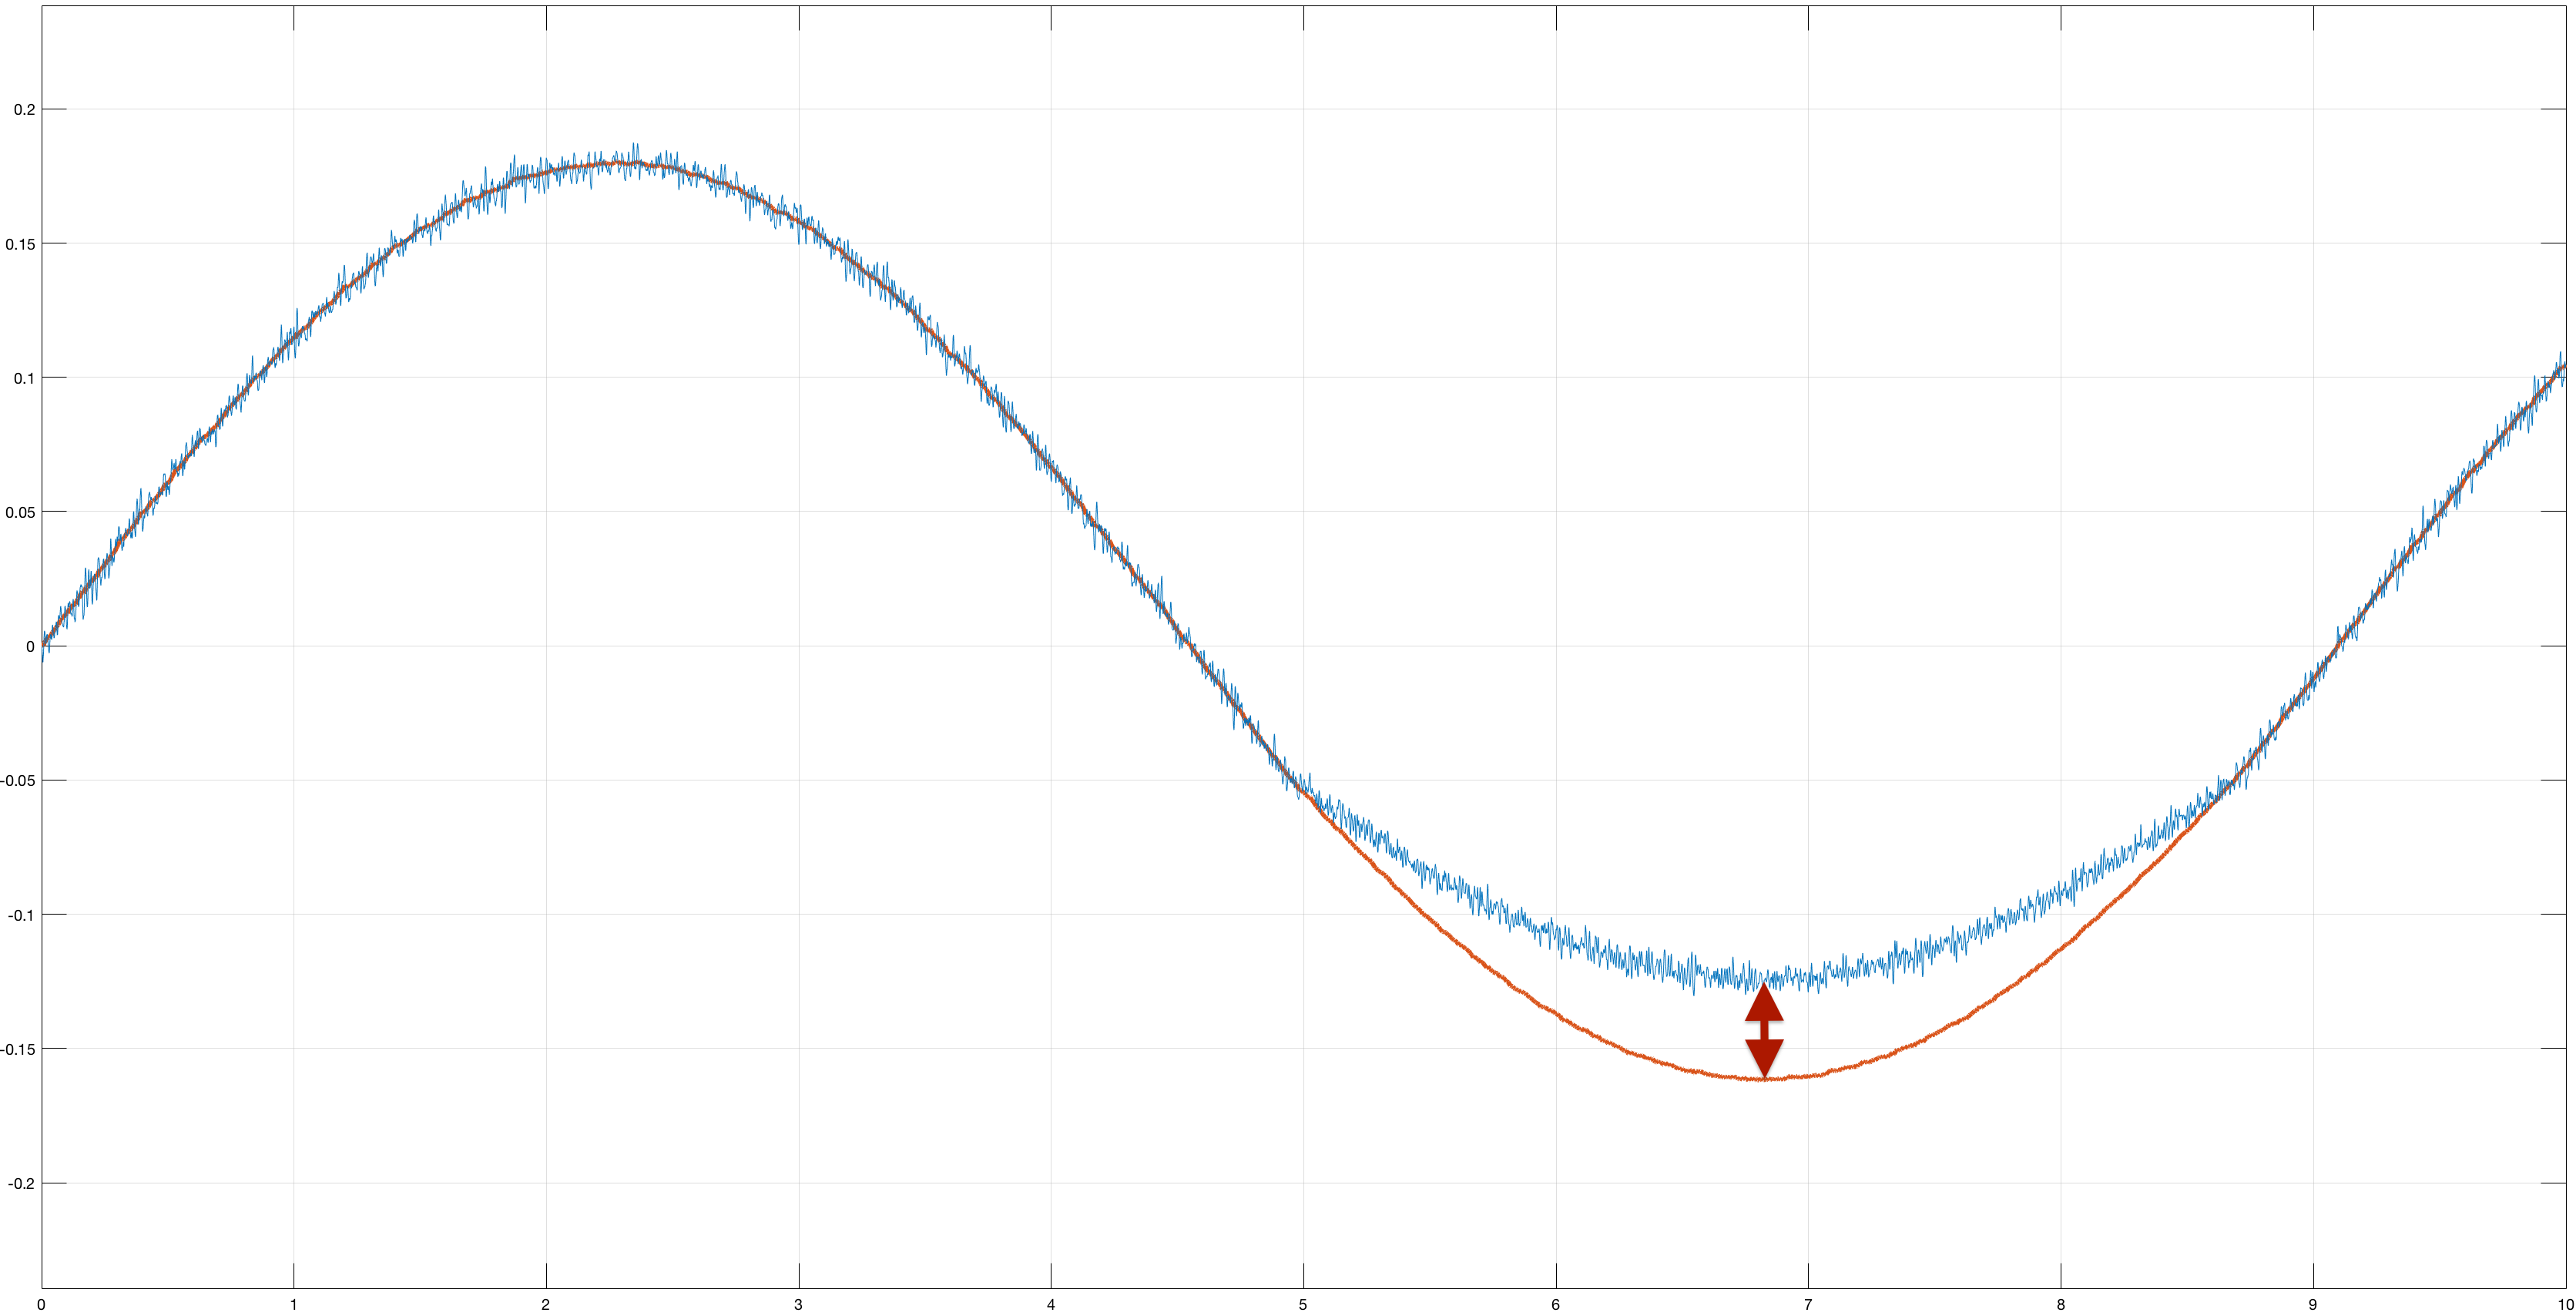
\includegraphics[width=\textwidth, height=0.45\textwidth]{Images/rigidContactReacPosArrow}
		\caption{ Angular position assumed during trajectory tracking.}
		\label{fig:ContactRigPos}
	\end{subfigure}	
\end{figure}
\begin{figure}[H]\ContinuedFloat
	\begin{subfigure}{1\linewidth}
		\centering
		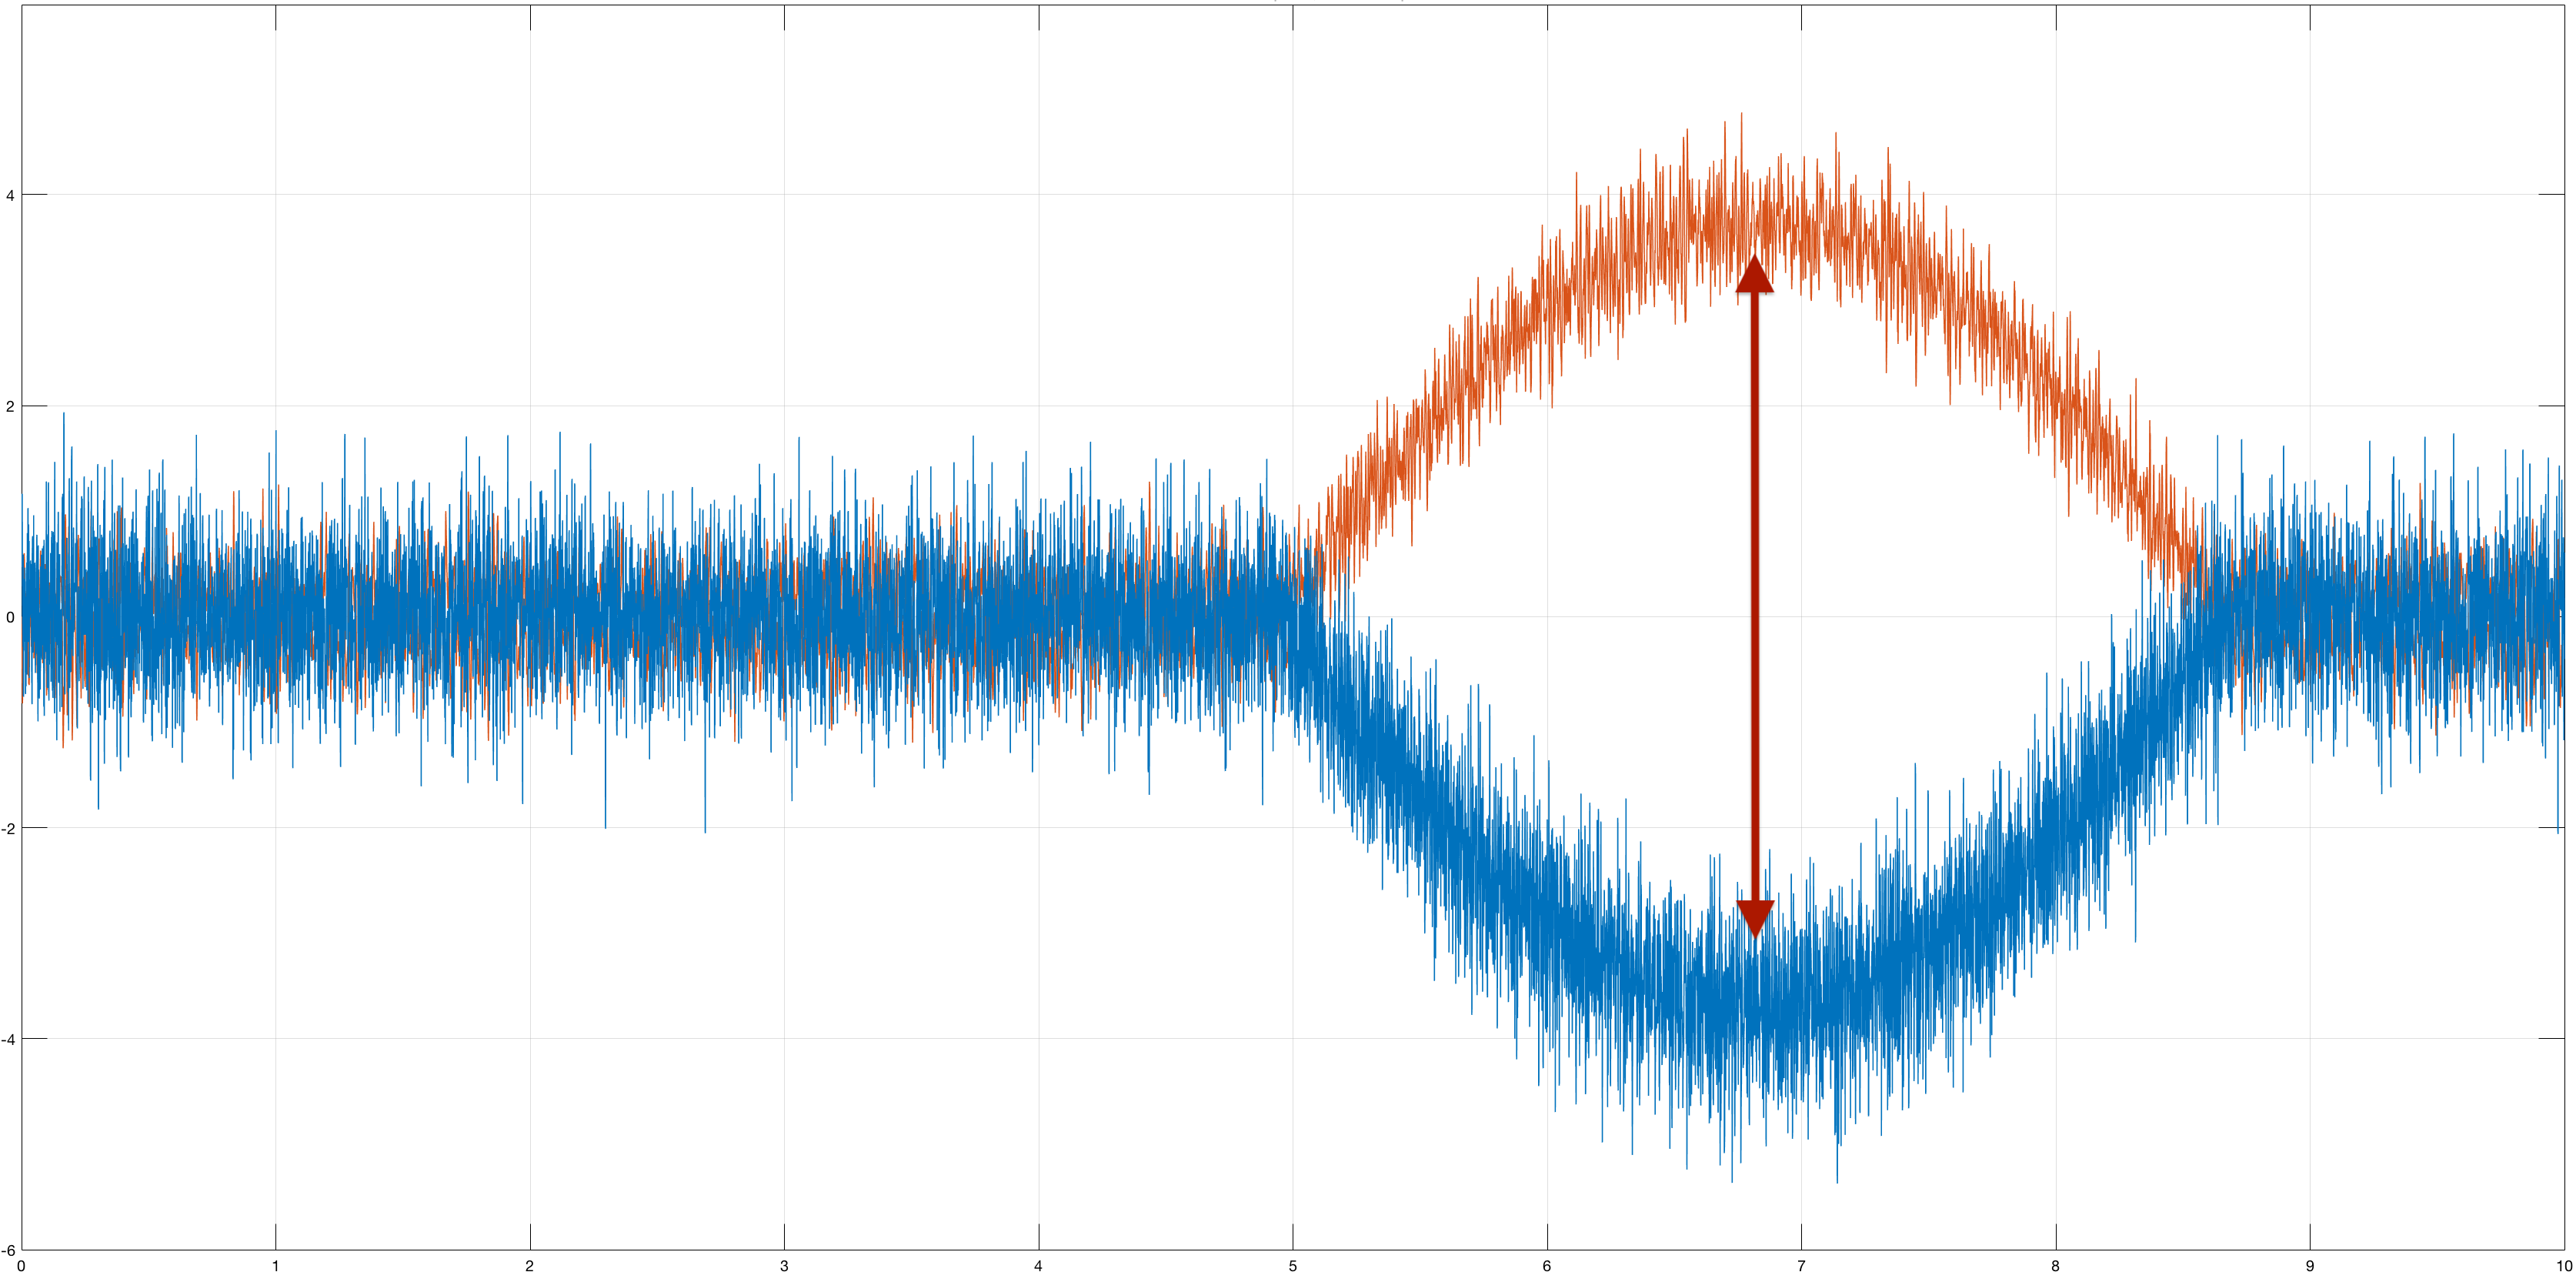
\includegraphics[width=\textwidth, height=0.45\textwidth]{Images/rigidContactReacTorArrow}
		\caption{ Torques exerted over time}
		\label{fig:ContactRigTor}
	\end{subfigure}	
  \caption{ Rigid coupling simulation in \textsl{contact} with the environment}
  \label{fig:contact_rigid}
\end{figure}

\newpage
\section{Conclusions}
Vibration suppression in the contest of bilateral teleoperation is an open
issue.

The proposed solution is based on a virtual spring-damper system with additional
inertia. The spring stiffness and the cut-off frequencies are chosen according to the system requirements.
\bigskip

To summarize, when the virtual stiffness has been fixed, the other virtual
parameters could be calculated from the equations in order to obtain the desired
cut-off frequencies.
\bigskip

The tracking error in free motion is similar using both \textbf{virtual compliance control} and \textbf{rigid coupling control}. However,the proposed controller shows promising results, since it preserves the useful (\textsl{low}) frequency inputs and reject the noisy ones (\textsl{high}). 
\bigskip
%Overall, the tracking error in free motion is almost null. And regarding the contact with the environment is interesting to observe from the simulations a trade-off between control effort and task error.

In contact motion the usage of the proposed controller leads to a position gab between master and slave and hence can be applied only to tasks that contemplate handling \textsl{soft} materials.



